\chapter{REVISÃO BIBLIOGRÁFICA}
\label{cap1Revisao}

Na América Latina, historicamente marcada por colônias de exploração, o extrativismo mineral teve início para atender aos interesses dos países colonizadores, continuando ao longo dos anos. No final da década de 1990, com a expansão da globalização e o aumento do consumo de metais, a indústria mineral começou a se expandir em ritmo acelerado, tanto em termos de volumes extraídos quanto na abertura de novas minas \cite{fernandes2016mineracao}.

Em 2023, o Brasil estava entre um dos principais produtores de minerais do mundo, ocupando a nona posição no ranking dos 20 principais países em termos de valor na produção de minerais metálicos e carvão \cite{wpr2024mineral}. Este setor possui significativa importância na economia nacional, gerando emprego e desempenhando um papel crucial nas exportações do país, com uma alta comercialização de commodities \cite{rbm2024mineracao}.

A atividade mineral apresenta potencial significativo para incrementar a arrecadação tributária e fomentar o crescimento econômico, além de proporcionar melhorias na qualidade de vida da população e promover o desenvolvimento regional, conforme argumentam \citeauthor{carvalho2012dependencia} (\citeyear{carvalho2012dependencia}, p. 1), o setor mineral possui relevância estratégica por sua presença em diversos segmentos econômicos, ``produzindo bens primários, que irão suprir as mais variadas atividades econômicas, desde a agricultura até indústrias de tecnologia de ponta''. Os autores ressaltam ainda, que
economias que possuem como base a extração dos recursos minerais têm a mineração como fator fundamental.

\section{Atividade de Mineração}
\label{sec:atividade_mineracao}

A história da mineração no território brasileiro remonta ao período colonial e se configura como um pilar fundamental na formação socioeconômica e política do país \cite{barreto2001, domingues2022}. A busca por riquezas minerais, inicialmente com o ouro no século XVIII, impulsionou a ocupação do território e moldou as primeiras estruturas de exploração \cite{barreto2001}. Contudo, é a partir do século XX que a relação entre o Estado e o setor mineral se institucionaliza de forma mais complexa, com a criação de códigos e regulamentos específicos para normatizar a atividade \cite{domingues2022}.

No início do século XX, o Estado brasileiro intensificou sua intervenção e regulamentação no setor mineral, culminando na promulgação de códigos específicos \cite{domingues2022}. Exemplos dessas intervenções incluem o Decreto Federal nº 24.642, de 10 de julho de 1934, que regulamenta o uso das jazidas na mineração \cite{brasil1934b}, o Decreto Federal nº 24.643, de 10 de julho de 1934, que trata da utilização das águas e continua em vigor até os dias atuais \cite{brasil1934c}, e o Código Florestal de 1934, estabelecido pelo Decreto Federal nº 23.793, de 23 de janeiro de 1934 \cite{brasil1934a}. 

O Código de Mineração de 1934 buscou consolidar a legislação existente e remover obstáculos para o aproveitamento racional das riquezas do subsolo \cite{brasil1934b}. Essa legislação conferiu ao Governo o papel de fiscalizar a execução dos planos de trabalho e orientar a marcha das atividades \cite{brasil1934b, domingues2022}, evidenciando uma preocupação crescente com o controle estatal sobre os recursos minerais. Essa intervenção legal e econômica do Estado no setor tornou-se uma marca da política mineral brasileira.

O arcabouço legal estabelecido pelo Código de 1934 definiu conceitos fundamentais e delineou o processo para a obtenção de direitos minerários \cite{brasil1934b}. Distinguiu-se formalmente ``jazida'', como a massa de substâncias minerais, de ``mina'', a jazida na extensão concedida e o conjunto de direitos associados à exploração \cite{brasil1934b}. O código classificou as jazidas, como por exemplo os minérios metálicos em jazidas primárias \cite{brasil1934b}, e instituiu a necessidade de autorização prévia para a pesquisa mineral \cite{barreto2001}. 

A concessão de lavra, ou seja, os trabalhos de extração e beneficiamento \cite{brasil1934b}, só seria outorgada após a pesquisa ter apresentado resultados satisfatórios e a jazida ser considerada lavrável pelo Departamento Nacional da Produção Mineral (DNPM) \cite{brasil1934b}. Essa estruturação legal visava garantir um aproveitamento mais ordenado das riquezas minerais.

A partir da década de 1930, sob o governo de Getúlio Vargas, a questão mineral foi integrada a um projeto nacionalista de desenvolvimento, visando à industrialização e à segurança nacional \cite{villasboas1995, fonseca2012, domingues2022}. Essa política representou uma ruptura estrutural nas relações entre o Estado e a economia, estabelecendo novos paradigmas para a autodeterminação do desenvolvimento nacional \cite{villasboas1995}. O setor mineral, reconhecido como estratégico para países em processo de industrialização, recebeu não apenas atenção prioritária, mas também investimentos significativos para sua expansão \cite{villasboas1995}.

Nesse período, foram criadas empresas estatais estratégicas para garantir o controle e o desenvolvimento de setores minerais considerados vitais para a economia nacional. A Companhia Vale do Rio Doce (CVRD) em 1942 e a Petrobrás em 1954 são exemplos dessa política estatal. Essa estratégia visava garantir o monopólio estatal para a exportação de minério de ferro e manganês e o regime estatal para a exploração da siderurgia, alinhando a política mineral à defesa econômica e militar da nação \cite{villasboas1995, fonseca2012}.

De acordo com \citeauthor{villasboas1995} \citeyear{villasboas1995}, a política nacionalista e intervencionista da era Vargas se contrapôs à visão liberal que defendia a maior participação do capital estrangeiro e a menor intervenção estatal na economia. O debate entre essas correntes ideológicas marcou a discussão sobre o caminho do desenvolvimento brasileiro, com o setor mineral frequentemente no centro das tensões. 

Enquanto a corrente nacionalista via o capital estrangeiro como complementar, desde que rigidamente controlado, a corrente liberal pregava a atração irrestrita de investimentos externos, mesmo para setores estratégicos. Essa polarização influenciou as decisões sobre o aproveitamento dos recursos minerais ao longo de décadas.

Após o segundo governo Vargas, especialmente durante o período de Juscelino Kubitschek (JK) e seu Plano de Metas, observou-se uma mudança na política econômica, com uma maior abertura e integração com o capital estrangeiro. Embora o período JK tenha focado no desenvolvimento industrial, a política econômica passou a fortalecer e expandir as bases de um ``capitalismo associado'', resultando em um aumento da importância das empresas associadas e multinacionais. Essa fase foi marcada por debates sobre a ``desnacionalização'' da economia e a crescente dependência, inclusive no setor mineral \cite{villasboas1995}.

O período da Ditadura Militar (1964-1985) manteve uma forte presença estatal no setor mineral e impulsionou grandes projetos, muitos deles voltados para a exportação e com participação de capital estrangeiro, especialmente na Amazônia \cite{fernandes2016, domingues2022}. Descobertas como o minério de ferro de Carajás (1967), a bauxita do Vale do Trombetas e a cassiterita de Pitinga exemplificam essa fase de expansão e direcionamento para o mercado global \cite{fernandes2016}. 

Os Códigos de Mineração de 1940 e 1967 \cite{brasil1967} representam marcos fundamentais neste processo de normatização e intervenção estatal no setor mineral brasileiro. Estas legislações estabeleceram um sofisticado sistema regulatório que, enquanto preservava elementos estruturais do ordenamento anterior, introduziu inovações significativas para atender às novas demandas desenvolvimentistas do país \cite{domingues2022}.

A partir da redemocratização, em 1985, o Brasil consolidou-se como um dos principais produtores e exportadores globais de minerais e metais. No período entre 1985 e 2015, o país exportava cerca de 85\% de sua produção mineral, com o minério de ferro constituindo a maior parte (89\%) dessa pauta exportadora. A mineração, juntamente com o agronegócio, tornou-se um setor estratégico para o equilíbrio da economia brasileira. Contudo, o forte direcionamento para a exportação de \emph{commodities} minerais, muitas vezes sem agregação de valor, e a concentração em poucos bens primários foram temas recorrentes na literatura \cite{fernandes2016}.

Na década de 1990, o conceito de desenvolvimento sustentável ganhou relevância nas discussões sobre a mineração no Brasil, impulsionado por reflexões globais e nacionais. O projeto Mineração, Minerais e Desenvolvimento Sustentável (MMSD - \emph{Mining, Minerals and Sustainable Development Project}), iniciado no final da década de 1990 sob a coordenação brasileira do Centro de Tecnologia Mineral (CETEM), constituiu uma iniciativa estratégica que objetivou construir um diagnóstico contemporâneo do setor mineral através do prisma da sustentabilidade. 

Esta abordagem inovadora permitiu uma reavaliação sistemática das práticas e políticas minerárias nacionais, estabelecendo novos parâmetros para a análise integrada do desenvolvimento sustentável na indústria extrativa, englobando também as dimensões econômica, institucional e social \cite{barreto2001}.

Um dos eixos centrais na discussão sobre mineração e desenvolvimento sustentável é a gestão dos impactos ambientais gerados pela atividade extrativa. A alteração da paisagem, a poluição da água e do solo, e a produção de grandes volumes de rejeitos são inerentes à natureza da mineração. Para mitigar esses efeitos, o gerenciamento ambiental tornou-se um instrumento crucial adotado pelas empresas, definido como o conjunto de técnicas e procedimentos para administrar demandas ambientais potencialmente geradoras de conflitos \cite{barreto2001}.

A promoção de tecnologias limpas e sustentáveis para otimizar o aproveitamento dos recursos, gerenciar rejeitos, minimizar impactos ambientais e maximizar a satisfação social é outro desafio fundamental. A efetivação de práticas mais sustentáveis na mineração brasileira exige um esforço contínuo para integrar as dimensões econômica, social e ambiental em todas as etapas do empreendimento. A jornada rumo a uma mineração verdadeiramente sustentável no Brasil, portanto, demanda a evolução contínua das políticas públicas, das práticas empresariais e do engajamento da sociedade civil \cite{barreto2001}.

Atualmente, o Brasil mantém-se como um dos principais produtores e exportadores de minérios do mundo: cerca de 80\% de tudo o que produz é exportado, gerando expressivo montante de divisas. Juntamente com o agronegócio, a mineração constitui-se um dos setores estratégicos para o equilíbrio da balança comercial brasileira. Apesar da diversificação crescente, o minério de ferro ainda representa aproximadamente 60\% das exportações do setor mineral brasileiro \cite{anm2023}.

Hoje, segundo o IBRAM \citeyear{ibram2024}, a indústria mineral do Brasil se destaca por:

\begin{itemize}
    \item Em 2024, o setor mineral registrou alta de 9,1\% no faturamento em relação a 2023, totalizando R\$ 270,8 bilhões (excluindo-se petróleo e gás);
    \item As exportações minerais brasileiras alcançaram US\$ 43,43 bilhões, um aumento de 0,9\%;
    \item As importações minerais caíram 23,1\% em US\$ (totalizando US\$ 8,5 bilhões) e 1,6\% em toneladas (totalização 41,2 milhões de toneladas);
    \item O saldo comercial mineral, de US\$ 34,9 bilhões equivale a 47\% do saldo comercial brasileiro, que foi de US\$ 74,5 bilhões;
    \item São mais de 221 mil empregos diretos no setor, desse total, foram geradas 8.703 novas vagas, no período de Janeiro e Novembro de 2024;
    \item As principais substâncias produzidas, com participação no faturamento do setor, são: Minério de ferro (59,35\%), Minério de ouro (8,81\%), minério de cobre (7,49\%), bauxita (2,11\%), água mineral (2,81\%), granito (2,81\%), calcário dolomítico (3,36\%), areia (1,36\%), fosfato (1,41\%), minério de níquel (0,83\%), minério de manganês (0,18\%), e minério de nióbio (0,44\%);
    \item Os principais Estados produtores em 2024, em bilhões R\$, e a participação dos mesmos no faturamento, respectivamente são: MG (R\$ 108,3; 40\%), PA (R\$ 97,6; 36,1\%), SP (R\$ 10,3; 3,8\%), BA (R\$ 10,1; 3,7\%), GO (R\$ 9,6; 3,6\%), MT (R\$ 7,5; 2,8\%), e outros (R\$ 27,4; 10,1\%).
\end{itemize}

\subsection{O papel da atividade mineradora na economia}
\label{subsec:papel_mineracao_economia}

\subsubsection{Percentual do PIB devido à mineração}
\label{subsubsec:percentual_pib}

A relevância de um setor produtivo na economia de um país é geralmente medida por sua contribuição ao produto interno bruto (PIB) \cite{leao2023}. A participação do setor mineral no Produto Interno Bruto (PIB) brasileiro constitui um elemento significativo para a compreensão da estrutura econômica nacional \cite{leao2023}. A mineração e a siderurgia representam conjuntamente aproximadamente 3,1\% do PIB nacional, com a mineração contribuindo isoladamente com cerca de 1,2\% e a siderurgia com 1,9\%, conforme demonstram os dados setoriais \cite{apc2024}. Entre os anos 2000 e 2019, essa participação oscilou entre 2,5\% e 4\%, refletindo tanto os ciclos econômicos internos quanto as flutuações nas cotações internacionais das commodities minerais, evidenciando a vulnerabilidade deste setor às dinâmicas do mercado global \cite{leao2023,ipea2023,apc2024}.

A mensuração precisa da contribuição econômica da cadeia produtiva mineral apresenta desafios metodológicos significativos devido à complexa interconexão entre diversos setores \cite{leao2023,ipea2023}. As abordagens tradicionais, que calculam apenas a participação direta no PIB, mostram-se insuficientes para capturar as vinculações setoriais diretas e indiretas que caracterizam a economia mineral. Estudos anteriores indicaram contribuições de aproximadamente 3,19\% do PIB em 2019, porém não contemplaram explicitamente o conceito de cadeia produtiva em sua totalidade. A delimitação do setor frequentemente baseia-se em critérios físicos de presença mineral nos produtos finais, metodologia que pode resultar em superdimensionamento setorial e dificulta o rastreamento preciso do impacto econômico mineral \cite{leao2023}.

A metodologia desenvolvida pelo Instituto de Pesquisa Econômica Aplicada (Ipea) e pelo Ministério de Minas e Energia (MME) em dezembro de 2023 trouxe avanços significativos para a análise econômica do setor mineral brasileiro. Este estudo, detalhado no trabalho de \citeonline{leao2023}, baseia-se na técnica de Matriz Insumo-Produto (MIP) adaptada para calcular o PIB sob o enfoque do valor adicionado, definindo a ``economia mineral'' como o conjunto das atividades extrativas e manufatureiras cuja função principal é transformar minerais em bens úteis. A metodologia permite capturar o ``arrasto produtivo'' --- a parcela do PIB gerada em outros setores econômicos que é estimulada pelas atividades centrais da economia mineral --- superando limitações de estudos anteriores e oferecendo uma visão mais abrangente da cadeia produtiva mineral.

Os resultados da aplicação desta metodologia revelam a dinâmica e extensão da cadeia produtiva mineral na economia brasileira ao longo de duas décadas \cite{leao2023}. A cadeia produtiva da economia mineral oscilou entre 2,5\% e 4,1\% do PIB brasileiro entre 2000 e 2019, representando entre R\$ 150 bilhões e R\$ 340 bilhões em valores constantes de 2021 \cite{apc2024}. A extração de minério de ferro destaca-se como setor-chave, apresentando capacidade de arrasto produtivo superior a 1 durante todo o período analisado, indicando que cada real de PIB gerado neste setor provoca mais de um real de PIB no restante da economia. O segmento de transformação mineral, especialmente a metalurgia de metais não ferrosos, também demonstrou expressivo poder multiplicador econômico, embora com trajetória mais volátil que a extração \cite{leao2023}.

\subsubsection{Mineração em números}
\label{subsubsec:mineracao_numeros}

Segundo dados da Mineração em Números \cite{ibram2023coletiva} apud \cite{fonseca2024resultados}, o setor apresentou os resultados abaixo, e que se encontram
representados nas Figuras \ref{fig:image1_mineracao_numeros_1}, \ref{fig:image2_mineracao_numeros_2} e \ref{fig:image3_mineracao_numeros_3}:

\begin{itemize}
\item O faturamento da indústria da mineração brasileira se manteve estável em 2023, em relação ao ano anterior, passando de R\$ 250 bilhões para R\$ 248,2 bilhões, uma redução de 0,7\%;

\item Minas Gerais aparece com a maior participação no faturamento: 41,7\% em 2023 -- passando de R\$ 100,5 bilhões em 2022 para R\$ 103,6 bilhões, (crescimento de 3\%).O Pará apresentou redução de 7,6\%, passando de R\$ 92,4 bilhões para R\$ 85,4 bilhões;

\item Entre as principais substâncias na participação do faturamento, destacam-se: minério de ferro (59,6\%) e ouro (8,5\%). Cobre (6,5\%), calcário (3,8\%), granito (2,6\%), bauxita (2,3\%) e nióbio (0,5\%) completam as substâncias de maior relevância;

\item As exportações minerais totais, tiveram alta de 3,1\% em relação a 2022, alcançando quase US\$ 43 bilhões, enquanto as importações minerais tiveram queda de 34,2\% (US\$ 11 bilhões);

\item O saldo comercial do setor, portanto, se situou em US\$ 31,95 bilhões, 28,3\% a mais do que em 2022 -- isso significa que o saldo mineral corresponde a 32\% do saldo total da balança comercial de 2023, que foi de US\$ 98,84 bilhões;

\item O minério de ferro respondeu por 71\% dos minérios exportados em 2023, passando de 344,1 milhões de toneladas em 2022 para 378,5 milhões de toneladas em 2023, um aumento de 10\%. As exportações do minério de ferro somaram US\$ 30,5 bilhões em 2023, registrando um aumento de 5,7\% frente aos US\$ 28,9 bilhões de 2022;

\item A coleta de impostos e encargos seguiu a tendência do volume de vendas em 2023. Houve uma diminuição de 0,7\%, com o montante passando de R\$ 86,2 bilhões em 2022 para R\$ 85,6 bilhões. A receita proveniente da Compensação Financeira pela Exploração Mineral (CFEM), que é o royalty do setor mineral, manteve-se
    praticamente constante, reduzindo de R\$ 7 bilhões para R\$ 6,9 bilhões de um ano para o outro;

\item Em termos de emprego, com 9 mil vagas a mais em 2023, o setor mineral manteve mais de 210 mil postos de trabalho diretos, conforme levantamento realizado em novembro de 2023 pelo Novo Caged, órgão vinculado ao Ministério do Trabalho e Emprego;

\item Destaca-se, ainda, o aumento nos aportes financeiros planejados pelas empresas mineradoras no país. Inicialmente projetados em US\$ 50 bilhões para o período de 2023 a 2027, os investimentos agora estão estimados em até US\$ 64,5 bilhões para o período de 2024 a 2028.

\item A sustentabilidade operacional está em foco nos investimentos. Até 2028, a indústria da mineração planeja aumentar em 62,7\% os recursos destinados a iniciativas socioambientais. Esses investimentos constituem a segunda maior proporção dos recursos setoriais previstos até 2028, correspondendo a 16,6\% do total, equivalente a US\$ 10,7 bilhões, comparados aos US\$ 6,6 bilhões projetados para o período de 2023 a 2027.
\end{itemize}

\begin{figure}[!htb]
    \centering
    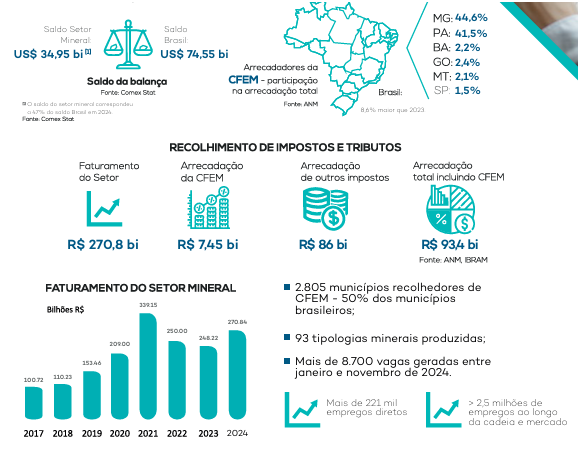
\includegraphics[width=\textwidth]{figures/image1_mineracao_numeros_1.png}
    \caption{Mineração em Números (2024) -- Saldo comercial, impostos e faturamento}
    \label{fig:image1_mineracao_numeros_1}
    \fonte{Mineração em Números (IBRAM, 2024)}
\end{figure}

\begin{figure}[!htb]
    \centering
    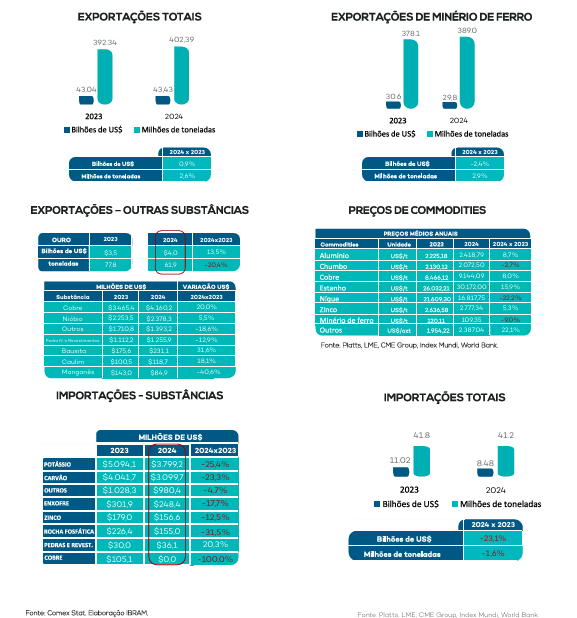
\includegraphics[width=\textwidth]{figures/image2_mineracao_numeros_2.png}
    \caption{Mineração em Números (2024) -- Exportação e Importação}
    \label{fig:image2_mineracao_numeros_2}
    \fonte{Mineração em Números (IBRAM, 2024)}
\end{figure}

\begin{figure}[!htb]
    \centering
    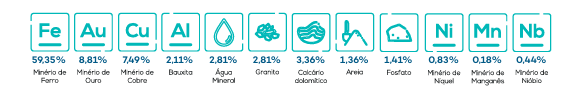
\includegraphics[width=\textwidth]{figures/image3_mineracao_numeros_3.png}
    \caption{Mineração em Números (2024) -- Principais substâncias produzidas -- Participação no faturamento do setor}
    \label{fig:image3_mineracao_numeros_3}
    \fonte{Mineração em Números (IBRAM, 2024)}
\end{figure}

\subsubsection{Geração de empregos}
\label{subsubsec:geracao_empregos}

A análise do mercado de trabalho no setor mineral brasileiro requer a delimitação das atividades econômicas relevantes, que, conforme metodologia da Agência Nacional de Mineração (ANM), abrangem a Indústria Extrativa Mineral (IEM) e a Indústria de Transformação Mineral (ITM). A IEM contempla atividades como extração de carvão mineral, minério de ferro, minerais metálicos e não metálicos, além de atividades de apoio, enquanto a ITM inclui a fabricação de produtos cerâmicos, artefatos de concreto, siderurgia, fundição, entre outras. Desde 2020, o monitoramento do emprego formal para o setor mineral, assim como para as demais atividades econômicas no Brasil, passou a ser realizado com base nos dados do Novo CAGED (eSocial), que substituiu o Cadastro Geral de Empregados e Desempregados (CAGED) e ampliou a base de trabalhadores formais avaliados \cite{anm2023c,anm2023d}. A análise conjunta ou separada dessas duas indústrias (IEM e ITM) é fundamental para entender a contribuição total do setor mineral para o emprego no país, o que será detalhado adiante.

\paragraph{Emprego Formal na Indústria Extrativa Mineral (IEM)}

O mercado de trabalho formal na Indústria Extrativa Mineral (IEM), excluindo petróleo e gás, é acompanhado trimestralmente pela ANM, evidenciando seu estoque de mão de obra e o saldo de contratações e desligamentos no período. No 3º trimestre de 2023, o estoque de trabalhadores da IEM no Brasil alcançou 208.447 postos (Figura \ref{fig:saldo_estoque_3tri2023}), enquanto no 4º trimestre de 2023, esse estoque foi de 208.176 postos (Figura \ref{fig:image5_saldo_estoque_4tri2023}). O saldo de emprego formal na IEM foi positivo no 3º trimestre de 2023, com 1.869 vagas criadas (Figura \ref{fig:saldo_estoque_3tri2023}), mas registrou uma leve variação negativa de -119 vagas no 4º trimestre de 2023 (Figura \ref{fig:image5_saldo_estoque_4tri2023}). Estes números refletem as flutuações na absorção de mão de obra direta pela atividade extrativa ao longo do ano \cite{anm2023c,anm2023d}.

\begin{figure}[!htb]
    \centering
    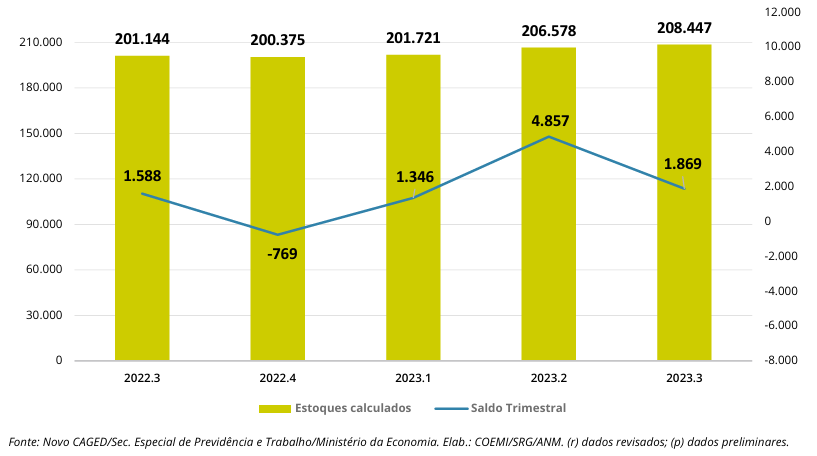
\includegraphics[width=\textwidth]{figures/image4_saldo_estoque_3tri2023.png}
    \caption{Saldo ajustado e estoque trimestral de mão de obra do setor de extração mineral (exceto petróleo e gás) -- 03TRI2023}
    \label{fig:saldo_estoque_3tri2023}
    \fonte{\citeauthor{anm2023c} (\citeyear{anm2023c})}
\end{figure}

\begin{figure}[!htb]
    \centering
    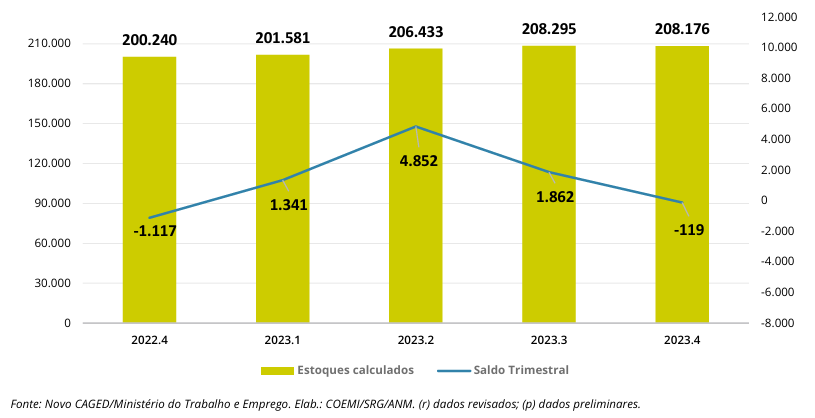
\includegraphics[width=\textwidth]{figures/image5_saldo_estoque_4tri2023.png}
    \caption{Saldo ajustado e estoque trimestral de mão de obra do setor de extração mineral (exceto petróleo e gás) -- 04TRI2023}
    \label{fig:saldo_estoque_4tri2023}
    \fonte{\citeauthor{anm2023d} (\citeyear{anm2023d})}
\end{figure}

As variações no saldo de emprego formal na IEM em 2023 foram influenciadas por dinâmicas distintas entre seus subgrupos, conforme a Classificação Nacional de Atividades Econômicas (CNAE 2.0) \cite{anm2023c,anm2023d}. No 3º trimestre de 2023, a Extração de Pedra, Areia e Argila apresentou um saldo positivo de 856 vagas, e a Extração de Minério de Ferro teve o maior saldo positivo, com 1.171 vagas (Figura \ref{fig:saldo_mao_obra_3tri2023}). Em contrapartida, a Extração de Minerais Metálicos Não-Ferrosos registrou um saldo negativo de -653 vagas no mesmo período, impactada pela suspensão das operações de extração de ouro pela AngloGold Ashanti em Santa Bárbara (MG), que resultou no encerramento de 754 postos de trabalho, e pela falência da Buritirama Mineração (manganês) em Marabá (PA), com fechamento de 408 postos \cite{anm2023c}. A variação interanual (4º trimestre de 2023 vs 4º trimestre de 2022) mostrou crescimento expressivo na Extração de Minério de Ferro (+12,7\%), mas quedas significativas nas Atividades de Apoio à Extração de Minerais (-38,6\%) e Extração de Outros Minerais Não-Metálicos (-5,3\%) (Figura \ref{fig:variacao_emprego_4tri2023}). Essas especificidades por subgrupo evidenciam a heterogeneidade da geração de emprego dentro da própria indústria extrativa.

\begin{figure}[!htb]
    \centering
    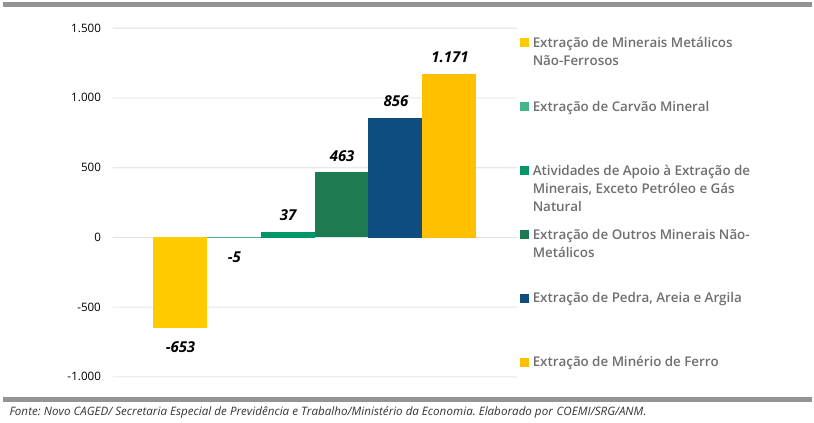
\includegraphics[width=\textwidth]{figures/image6_saldo_mao_obra_3tri2023.png}
    \caption{Saldo de mão de obra da indústria extrativa mineral (exceto petróleo e gás), por grupo CNAE 2.0 -- 03TRI2023}
    \label{fig:saldo_mao_obra_3tri2023}
    \fonte{\citeauthor{anm2023c} (\citeyear{anm2023c})}
\end{figure}

\begin{figure}[!htb]
    \centering
    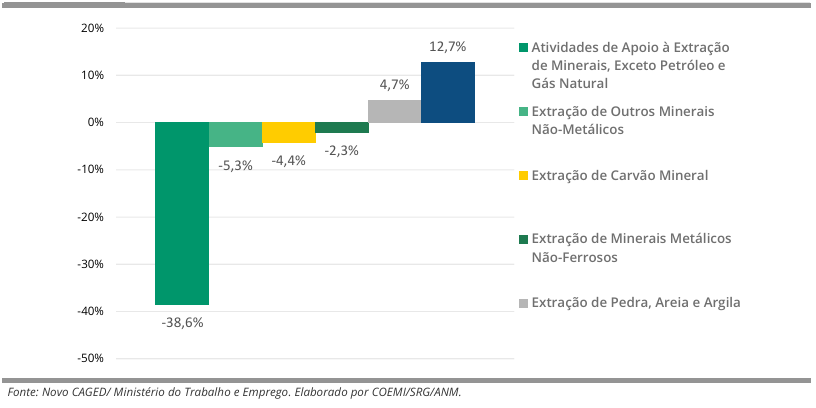
\includegraphics[width=\textwidth]{figures/image7_variacao_emprego_4tri2023.png}
    \caption{Variação interanual do emprego formal na indústria extrativa (exceto petróleo e gás), por grupo CNAE 2.0 -- 04TRI2023}
    \label{fig:variacao_emprego_4tri2023}
    \fonte{\citeauthor{anm2023d} (\citeyear{anm2023d})}
\end{figure}

A maior parte da distribuição da força de trabalho da IEM está concentrada nos estados de Minas Gerais (35\%), Pará (13\%), Bahia (7\%) e São Paulo (7\%) (Figura \ref{fig:estoque_mao_obra}) \cite{anm2023}.

\begin{figure}[!htb]
    \centering
    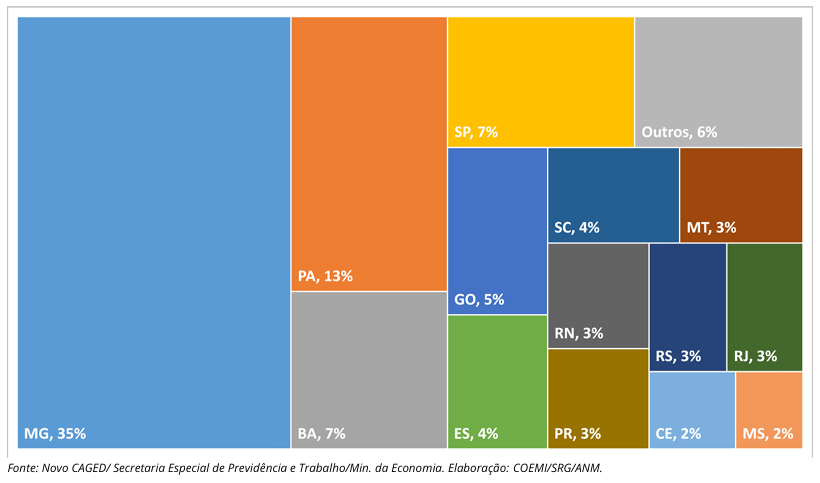
\includegraphics[width=\textwidth]{figures/image8_estoque_mao_obra.png}
    \caption{Estoque de mão de obra da IEM (exceto petróleo e gás) por estado}
    \label{fig:estoque_mao_obra}
    \fonte{\citeauthor{anm2023c} (\citeyear{anm2023c})}
\end{figure}

\paragraph{Indústria de Transformação Mineral (ITM)}

Por outro lado, a Indústria de Transformação Mineral (ITM) concentra a maior parte da mão de obra formal do setor mineral brasileiro, apresentando um estoque de trabalhadores significativamente superior ao da indústria extrativa \cite{anm2023c,anm2023d}. No 4º trimestre de 2023, a ITM registrou 718.631 postos de trabalho (Figura \ref{fig:evolucao_saldo_itm}), enquanto no 3º trimestre de 2023, o estoque era de 655.078 postos (Figura \ref{fig:evolucao_saldo_itm_3tri}). Os principais setores empregadores dentro da ITM são a Fabricação de Produtos Cerâmicos, Fabricação de Artefatos de Concreto, Cimento, Fibrocimento, Gesso e Materiais Semelhantes, Aparelhamento de Pedras e Fabricação de Outros Produtos de Minerais Não Metálicos, e Siderurgia \cite{anm2023c,anm2023d}. Embora o estoque de mão de obra na ITM seja maior, sua variação trimestral tem sido discreta, como a leve queda de 0,3\% no 4º trimestre de 2023 em relação ao mesmo trimestre de 2022, indicando uma estabilidade relativa em comparação com as flutuações mais acentuadas observadas em alguns grupos da IEM.

\begin{figure}[!htb]
    \centering
    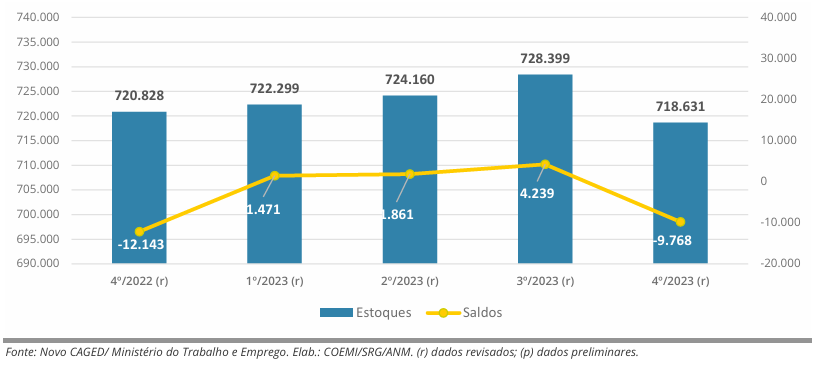
\includegraphics[width=\textwidth]{figures/image10_evolucao_saldo_itm.png}
    \caption{Evolução do saldo e do estoque de trabalhadores da ITM -- 04TRI2022 a 04TRI2024}
    \label{fig:evolucao_saldo_itm}
    \fonte{\citeauthor{anm2023d} (\citeyear{anm2023d})}
\end{figure}

\begin{figure}[!htb]
    \centering
    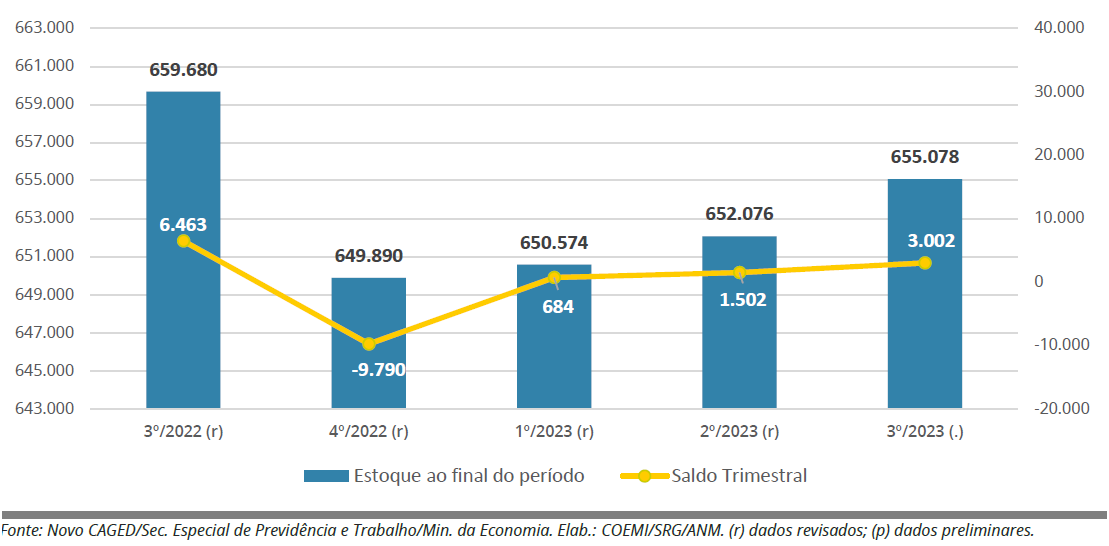
\includegraphics[width=\textwidth]{figures/image10_evolucao_saldo_itm_3tri.png}
    \caption{Evolução do saldo e do estoque de trabalhadores da ITM -- 03TRI2022 a 03TRI2024}
    \label{fig:evolucao_saldo_itm_3tri}
    \fonte{\citeauthor{anm2023c} (\citeyear{anm2023c})}
\end{figure}

Apesar da menor quantidade de postos de trabalho diretos na IEM em comparação com a ITM, essa indústria extrativa se destaca pela geração de rendimentos elevados para seus trabalhadores. A mediana dos salários de admissão na Indústria Extrativa Mineral, considerando todos os grupos CNAE 2.0 exceto petróleo e gás, foi de R\$ 1.988,67 no 4º trimestre de 2023. Salários medianos mais altos foram observados em grupos específicos como Extração de Carvão Mineral (R\$ 3.370,31), Extração de Minério de Ferro (R\$ 2.300,43) e Extração de Minerais Metálicos Não-Ferrosos (R\$ 2.250,00) no mesmo período (Figura \ref{fig:salarios_admissao}). Esta característica de alta remuneração por posto de trabalho direto reforça a contribuição econômica do setor, que vai além da mera quantidade de empregos gerados \cite{anm2023d}.

\begin{figure}[!htb]
    \centering
    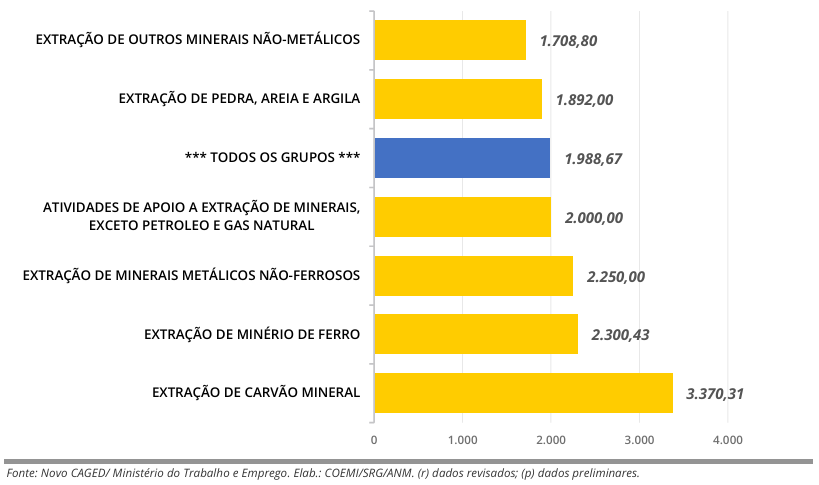
\includegraphics[width=\textwidth]{figures/image11_salarios_admissao.png}
    \caption{Salários de admissão na extração mineral na IEM -- 04TRI2023}
    \label{fig:salarios_admissao}
    \fonte{\citeauthor{anm2023d} (\citeyear{anm2023d})}
\end{figure}

Complementarmente, a Indústria Extrativa Mineral contribui de forma expressiva para as finanças públicas por meio da Compensação Financeira pela Exploração de Recursos Minerais (CFEM), um royalty devido pela utilização econômica dos recursos minerais \cite{anm2023a}. No 3º trimestre de 2023, a arrecadação da CFEM totalizou R\$ 1,76 bilhão \cite{anm2023c}, enquanto no 4º trimestre de 2023, foi de R\$ 1,80 bilhão \cite{anm2023d}, em valores nominais. Os estados de Minas Gerais e Pará concentram a maior parte da arrecadação da CFEM, respondendo por 85,4\% no 3º trimestre de 2023 \cite{anm2023c} e 87,4\% no 4º trimestre de 2023 \cite{anm2023d}, com destaque para municípios como Parauapebas (PA) e Canaã dos Carajás (PA) \cite{anm2023c,anm2023d}. O minério de ferro é a substância mineral que mais contribui para a CFEM \cite{anm2023c,anm2023a}. Estes recursos fiscais, gerados diretamente pela atividade extrativa, representam um potencial significativo para investimento em desenvolvimento local e regional.

Baseada nos informes recentes da ANM, a análise corrobora que a Indústria Extrativa Mineral no Brasil, embora menos intensiva em mão de obra direta em comparação com a Indústria de Transformação Mineral, gera postos de trabalho com rendimentos acima da média e contribui substancialmente para a arrecadação fiscal via CFEM. A dinâmica do emprego direto na IEM é granular e sujeita a eventos específicos em subgrupos de substâncias, como observado nos saldos trimestrais de 2023. A ITM, por sua vez, mantém um estoque de mão de obra maior e mais estável. Portanto, a análise da geração de emprego na mineração brasileira deve considerar a dualidade entre a natureza da extração e da transformação, bem como o potencial de encadeamento e investimento decorrente da alta geração de valor e tributos da indústria extrativa \cite{anm2023c,anm2023d}.

\subsection{Geração de resíduos}
\label{subsec:geracao_residuos}

Nessa sessão apresenta-se uma visão da geração de resíduos minerais.

\subsubsection{Etapas da Mineração}
\label{subsubsec:etapas_da_mineracao}

A atividade de mineração compreende um conjunto de processos técnicos e operacionais, conforme estabelecido pelo Decreto nº 9.406/2018, Art. 5º, que incluem pesquisa geológica, desenvolvimento da mina, lavra, beneficiamento dos minérios, transporte, comercialização, gestão (aproveitamento) de resíduos, o armazenamento de estéreis e rejeitos e o fechamento da mina \cite{brasil2018}.

Esse processo é geralmente dividido em etapas sequenciais que orientam o planejamento e a execução dos empreendimentos. As principais fases identificadas na literatura (Figura \ref{fig:etapas_mineracao}) incluem a Prospecção, a Pesquisa Mineral, a Lavra e o Descomissionamento/Fechamento da Mina. Outras atividades cruciais como o Beneficiamento, a Comercialização e o aproveitamento de resíduos são por vezes incluídas no ciclo ou consideradas partes da Lavra ou etapas subsequentes \cite{carvalho2018, freire2020}.

\begin{figure}[!htb]
    \centering
    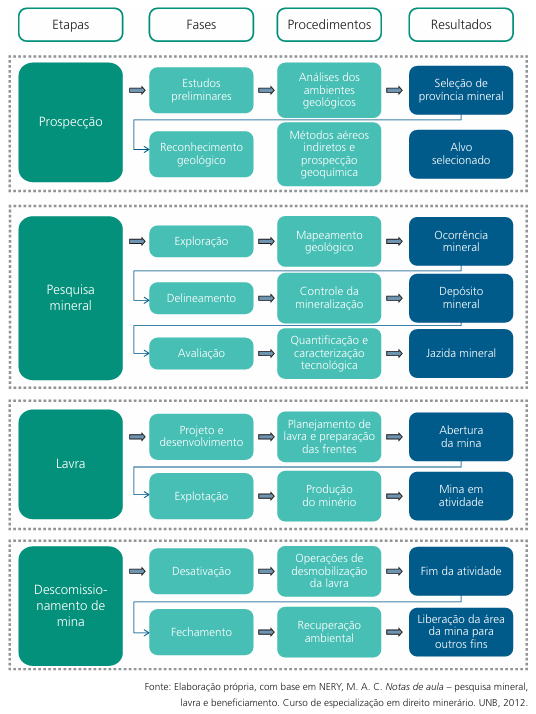
\includegraphics[width=0.9\textwidth]{figures/image14_etapas_mineracao.png}
    \caption{Etapas da mineração.}
    \label{fig:etapas_mineracao}
    \fonte{\citeauthor{carvalho2018} (\citeyear{carvalho2018})}
\end{figure}

A seguir, são descritos os processos e as atividades associadas a cada etapa, com ênfase particular nas fases de lavra e descomissionamento de mina, devido ao seu significativo impacto nos ambientes mineiros \cite{carvalho2018}.

A Prospecção constitui a fase inicial do ciclo, focada na busca por concentrações de minério de interesse econômico. Nesta etapa, são realizados estudos preliminares e reconhecimento geológico da área, que podem incluir análises de ambientes geológicos, métodos aéreos indiretos e prospecção geoquímica. O principal resultado da prospecção é a seleção de províncias minerais e alvos potenciais para investigações mais aprofundadas. Embora inicial, essa fase já pode gerar aspectos ambientais como mapeamento e estudos de campo, e potenciais impactos adversos como especulação financeira e pressão sobre propriedades \cite{freire2020}.

Após a identificação de alvos promissores, segue-se a fase de Pesquisa Mineral, que visa caracterizar a ocorrência mineral, o depósito e a jazida. Procedimentos como mapeamento geológico, exploração, delineamento e avaliação são conduzidos para controlar a mineralização, quantificar e caracterizar tecnologicamente o material encontrado. Esta fase é fundamental para determinar a exequibilidade econômica do aproveitamento da jazida \cite{freire2020}. A pesquisa mineral precede a fase de lavra e é regulada pelo Regime de Autorização \cite{anm2022}.

A lavra constitui o conjunto de operações coordenadas que visam o aproveitamento industrial de uma jazida, englobando desde a extração das substâncias minerais úteis até o seu beneficiamento \cite{jr2019}. Conforme estabelecido pelo Código Brasileiro de Mineração \cite{brasil1967}, essa fase essencial da mineração abarca diversas atividades (Figura \ref{fig:operacoes_lavra}), como o projeto e desenvolvimento da mina, a preparação das frentes de lavra, a abertura da mina e a extração do minério, culminando no beneficiamento \cite{carvalho2018, freire2020}. Reconhecida como a etapa mais intensiva na geração de efluentes, sejam eles sólidos, líquidos ou gasosos \cite{carvalho2018, freire2020}, a lavra representa o ponto central do ciclo produtivo mineral. A complexidade das operações de lavra exige uma análise cuidadosa das características do depósito mineral e dos fatores externos para a seleção do método mais adequado.

\begin{figure}[!htb]
    \centering
    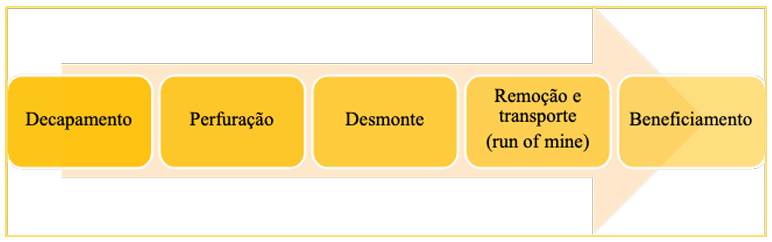
\includegraphics[width=0.9\textwidth]{figures/image16_operacoes_lavra.png}
    \caption{Operações de lavra.}
    \label{fig:operacoes_lavra}
    \fonte{\citeauthor{carvalho2018} (\citeyear{carvalho2018}), p. 344 apud \citeauthor{freire2020} (\citeyear{freire2020})}
\end{figure}

Por envolver atividades com alto impacto ambiental, o início da etapa de lavra depende, em geral, de estudo de impacto ambiental (EIA), e seu respectivo relatório de impacto ambiental (Rima), e da licença ambiental dos órgãos competentes \cite{carvalho2018}.

A escolha do método de lavra é um fator determinante para o sucesso da operação de extração e é intrinsecamente limitada pelas características físicas do depósito mineral. Fatores como profundidade, extensão e inclinação do corpo mineralizado são primordiais para delinear as possibilidades de aplicação dos diferentes métodos de lavra \cite{carvalho2018}. Além das condições geológicas intrínsecas à jazida, uma série de outros aspectos devem ser considerados no planejamento, incluindo a relação estéril-minério, a segurança das operações, a viabilidade econômica do empreendimento e critérios geológicos, sociais, geográficos e ambientais. A estabilidade da mina, a máxima recuperação do minério e a produtividade máxima também são elementos cruciais que orientam a decisão sobre qual técnica de lavra será implementada. Com base nesses fatores e nas características da jazida, a lavra é classificada em dois grandes grupos principais \cite{carvalho2018, jr2019}.

De acordo com \cite{jr2019}, esse processo é classificado em dois grandes grupos: lavra subterrânea e superficial (a céu aberto). Esta classificação baseia-se nas distintas técnicas de extração do minério, denominadas métodos de lavra, utilizadas em cada grupo (Figura \ref{fig:metodos_lavra}).

\begin{figure}[!htb]
    \centering
    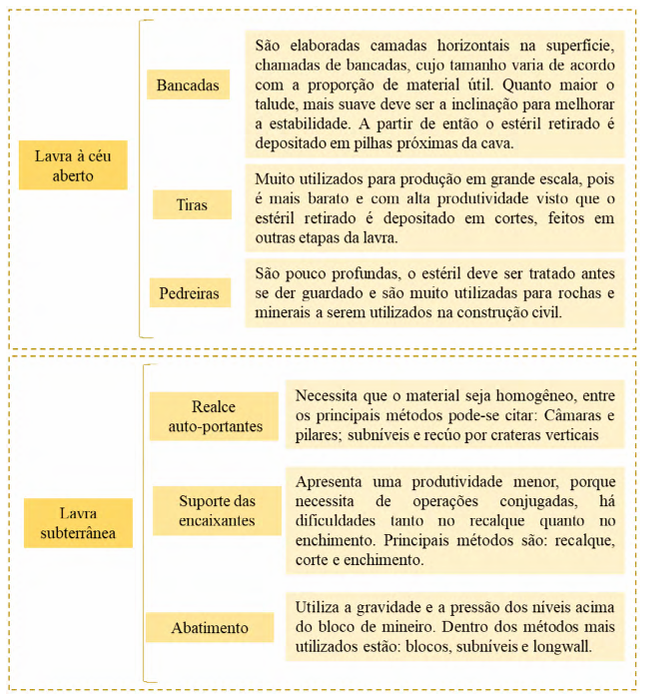
\includegraphics[width=0.9\textwidth]{figures/image15_metodos_lavra.png}
    \caption{Métodos de Lavra.}
    \label{fig:metodos_lavra}
    \fonte{\citeauthor{jr2019} (\citeyear{jr2019}) apud \citeauthor{freire2020} (\citeyear{freire2020})}
\end{figure}

Um dos grandes grupos de métodos é a lavra a céu aberto, também conhecida como lavra superficial, que se caracteriza pela extração do material mineral diretamente em uma escavação realizada na superfície terrestre \cite{jr2019, freire2020}. Este método é tipicamente indicado para depósitos minerais que se encontram próximos à superfície, apresentando estrutura, mergulho, espessura e forma que favoreçam o acesso e a extração por meio de escavações abertas. As operações de lavra a céu aberto frequentemente envolvem a remoção de camadas de material estéril que recobrem o corpo de minério. Após a extração, o material passa por etapas subsequentes de manuseio e processamento \cite{freire2020}. No Brasil, a maioria das minas opera a céu aberto \cite{carvalho2018, freire2020}, sendo regida pelo Regime de Concessão \cite{anm2022}.

O outro grande grupo de métodos de lavra é a lavra subterrânea, que, diferentemente da lavra a céu aberto, realiza a extração do minério abaixo da superfície terrestre. O acesso ao corpo de minério em uma mina subterrânea é feito através da abertura de poços, túneis e galerias, que se desenvolvem nas rochas encaixantes. Este método é usualmente adotado quando a profundidade do depósito mineral torna a lavra a céu aberto inviável economicamente ou logisticamente. A complexidade e os custos da lavra subterrânea são geralmente maiores do que os da lavra a céu aberto, mas permitem o acesso a jazidas localizadas em maiores profundidades. A decisão entre esses dois métodos principais é um ponto crítico no planejamento da mina \cite{jr2019, freire2020}.

Dentro da fase de Lavra, processos como Desmonte da Rocha, Carregamento e Transporte são essenciais. O desmonte envolve a extração mineral, frequentemente utilizando técnicas como perfuração e detonação. O material desmontado, chamado de \textit{run of mine} (ROM), é então carregado e transportado para a unidade de beneficiamento, geralmente localizada próxima à mina ou para pilhas de deposição. Estes procedimentos envolvem grande movimentação de material e equipamentos pesados, gerando impactos ambientais como ruído, emissões atmosféricas e alteração da paisagem \cite{carvalho2018, freire2020}.

O Beneficiamento (ou Tratamento ou Produção) é um processo fundamental, muitas vezes considerado etapa integrante do conjunto de operações de Lavra, que se realiza sobre o ROM \cite{carvalho2018}. O objetivo é separar fisicamente os minerais úteis da ganga (a parte sem interesse econômico), utilizando uma série de processos que podem incluir fragmentação (britagem, moagem), classificação (peneiramento), concentração (separação magnética, flotação) e desaguamento \cite{freire2020}. Este processo gera uma grande quantidade de resíduos finos e ultrafinos, conhecidos como rejeitos, que, misturados à água do processo, formam a polpa (lama) de rejeito. A quantidade e as características dos rejeitos variam significativamente dependendo do tipo de minério, da composição da jazida e dos processos de beneficiamento adotados \cite{ibram2016}.

As fases finais do ciclo incluem o Armazenamento, Distribuição e Comercialização dos produtos minerais. O material beneficiado (concentrado) é armazenado e preparado para distribuição e venda. A comercialização é a etapa onde o produto final alcança o mercado, gerando valor econômico e impostos. Embora voltadas para o produto final, essas fases também podem gerar impactos ambientais associados ao transporte e à infraestrutura necessária. O Brasil é um grande produtor de minério de ferro, com destino principal para a China \cite{freire2020}.

Finalmente, o ciclo culmina com o Descomissionamento e Fechamento da Mina. Esta fase envolve a desativação das operações, desmobilização de equipamentos e instalações, e a recuperação ambiental da área impactada \cite{carvalho2018}. O objetivo é devolver o local para outros usos pela comunidade, minimizando os riscos ambientais de longo prazo. O plano de fechamento deve ser elaborado e atualizado periodicamente, e o monitoramento dos efeitos posteriores, mesmo após a reabilitação inicial, é crucial para a segurança e sustentabilidade \cite{lozano2006}.

\subsubsection{Resíduos sólidos de extração - Estéril}

A atividade de mineração, conforme delineada acima, compreende diversas etapas que intrinsecamente geram materiais residuais, destacando-se entre eles o estéril e os rejeitos. O estéril é o material sólido removido durante a extração mineral (como o decapeamento superficial ou a retirada da sobrecarga) que não possui valor econômico. Geralmente mantidos na própria mina em forma de pilhas ou utilizados estrategicamente para o preenchimento de cavas exauridas. O volume de estéril produzido é influenciado pelas características geológicas da região, pela concentração da substância mineral na rocha matriz e pela localização da jazida. Este volume é determinado pela razão de estéril/minério, que representa a relação entre a quantidade de estéril a ser removida e a quantidade de minério bruto lavrado \cite{freire2020}; essa produção bruta de minério, frequentemente referida como Run-of-Mine (ROM), representa a quantidade total de minério extraído diretamente da mina em um determinado ano, sem passar por qualquer processo de beneficiamento ou tratamento \cite{anm2022}. Por regulamentação, os relatórios anuais de atividades mineradoras devem detalhar a relação observada entre a substância útil e o estéril, conforme estabelecido pela legislação brasileira \cite{brasil1967}.

\subsubsection{Resíduos sólidos de beneficiamento - Rejeito}

A atividade de mineração, em sua essência, compreende um conjunto de operações que vão desde a extração das substâncias minerais úteis até o seu beneficiamento. O rejeito é a porção do minério bruto que é descartada após passar pelo processo de beneficiamento ou tratamento. Este material geralmente não tem valor econômico nas condições vigentes, possuem características variáveis conforme o tipo de mineral processado e os métodos mecânicos e/ou químicos empregados no beneficiamento, e frequentemente se apresenta misturado à água, formando uma polpa \cite{freire2020}.

Os rejeitos podem apresentar-se em duas formas principais: rejeitos finos, compostos por siltes (partículas com diâmetro entre 4 $\mu$m e 64 $\mu$m segundo a escala de Wentworth, ou conforme a NBR 6502 da ABNT, solo com baixa ou nenhuma plasticidade e reduzida resistência quando seco), geralmente depositados na forma de lama ou polpa; e rejeitos granulares, com granulometria mais grossa e características arenosas. A distinção entre estas categorias é significativa do ponto de vista geotécnico, pois os rejeitos granulares apresentam elevada permeabilidade, resistência significativa ao cisalhamento e eficiente capacidade de sedimentação, facilitando sua estabilização em depósitos, enquanto os rejeitos finos apresentam desafios consideráveis no processo de sedimentação \cite{carvalho2018}.

O material residual proveniente do beneficiamento mineral pode ser disposto mediante duas modalidades distintas: na forma de material granular sólido, cuja transferência ocorre por meio de caminhões ou correias transportadoras; ou na forma de polpa (composta por partículas sólidas em meio aquoso), a qual é conduzida através de sistemas tubulares, valendo-se de mecanismos de bombeamento hidráulico ou do princípio físico do gradiente gravitacional \cite{duarte2008}.

A quantidade gerada está diretamente associada não apenas à concentração do mineral útil na rocha matriz, mas também ao método de lavra empregado, que influencia a geração de efluentes sólidos, líquidos e gasosos. A adequada gestão destes materiais residuais representa um desafio histórico para o setor minerário \cite{carvalho2018}.

\subsubsection{Geração de resíduos sólidos (Sólidos, líquidos, gasosos)}

A mineração, desde a extração das substâncias minerais úteis até o seu beneficiamento, gera invariavelmente uma grande quantidade de resíduos sólidos. Esses resíduos são principalmente categorizados como estéril e rejeito \cite{freire2020}.

No Brasil, as substâncias metálicas possuem grande importância na indústria mineral, respondendo por cerca de 82\% do valor total da produção mineral em 2022 \cite{anm2023a} e cerca de 89\% em 2021 \cite{anm2022}. Onze substâncias metálicas destacam-se por constituírem a ampla maioria do valor econômico da produção mineral brasileira, representando mais de 99\% do valor total gerado nesta classe de recursos. Estas substâncias são: alumínio (extraído da bauxita), cobre, cromo, estanho, ferro, manganês, nióbio, níquel, ouro, vanádio e zinco \cite{anm2023a}.

A produção bruta, beneficiada e comercializada dos principais minerais metálicos no Brasil está apresentada na Tabela~\ref{tab:mineral-production}, que consolida os dados de 2023.

\begin{table}[ht]
    \centering
    \caption{Produção Bruta, Beneficiada e Comercializada - Principais Substâncias Metálicas 2023}
    \resizebox{\textwidth}{!}{
    \begin{tabular}{|l|rr|rr|rr|rr|r|}
    \hline
    \multirow{3}{*}{\textbf{Substância}} & \multicolumn{2}{c|}{\textbf{Produção Bruta}} & \multicolumn{2}{c|}{\textbf{Produção Beneficiada}} & \multicolumn{4}{c|}{\textbf{Produção Comercializada}} & \multirow{3}{*}{\textbf{Valor Total (R\$)}} \\
    \cline{6-9}
     & \multicolumn{2}{c|}{} & \multicolumn{2}{c|}{} & \multicolumn{2}{c|}{\textbf{Bruta}} & \multicolumn{2}{c|}{\textbf{Beneficiada}} & \\
    \cline{2-9}
     & \textbf{Quantidade (ROM)} & \textbf{Teor (\%)} & \textbf{Quantidade} & \textbf{Teor (\%)} & \textbf{Quantidade} & \textbf{Valor (R\$)} & \textbf{Quantidade} & \textbf{Valor (R\$)} & \\
    \hline
    Alumínio (Bauxita) & 44.245.579 & 41,00 & 31.608.694 & 48,00 & 1.214.221 & 52.167.556 & 31.753.849 & 5.736.766.460 & 5.788.934.016 \\
    \hline
    Chumbo & 2.971.893 & 1,14 & 29.417 & 28,23 & - & - & 26.718 & 167.202.096 & 167.202.096 \\
    \hline
    Cobre & 84.627.605 & 0,55 & 1.024.418 & 35,38 & 5.194 & 3.312.424 & 1.038.309 & 14.252.345.082 & 14.255.657.506 \\
    \hline
    Columbita-Tantalita & 0 & - & 10.977 & 34,52 & - & - & 10.400 & 237.870.337 & 237.870.337 \\
    \hline
    Cromo & 1.424.312 & 17,11 & 565.575 & 38,66 & - & - & 570.450 & 479.264.446 & 479.264.446 \\
    \hline
    Estanho & - & - & 28.167.100 & 68,08 & - & - & 29.878.602 & 1.931.850.703 & 1.931.850.703 \\
    \hline
    Ferro & 554.089.729 & 53,96 & 411.681.935 & 62,41 & 56.820.207 & 1.342.784.848 & 400.193.563 & 161.228.089.878 & 162.570.874.726 \\
    \hline
    Grafita & 799.100 & 5,11 & 72.780 & - & 187.189 & 4.296.564 & 66.352 & 433.404.413 & 437.700.977 \\
    \hline
    Lítio & 900.757 & 1,06 & 143.720 & 4,88 & - & - & 143.634 & 1.736.369.463 & 1.736.369.463 \\
    \hline
    Manganês & 2.275.200 & 35,18 & 1.172.511 & 38,81 & 147.310 & 58.851.555 & 927.079 & 387.119.456 & 445.971.011 \\
    \hline
    Nióbio & 14.758.997 & 1,29 & 200.940 & 52,52 & - & - & 119.404 & 1.071.873.989 & 1.071.873.989 \\
    \hline
    Níquel & 12.392.049 & 0,87 & 360.616 & 17,77 & 113.647 & 28.605.629 & 362.082 & 9.042.426.931 & 9.071.032.560 \\
    \hline
    Ouro - Concessão & 67.199.488 kg & 0,99 g/t & 57.376 kg & 99,46\% & - & - & 58.511 kg & 16.538.812.304 & 16.538.812.304 \\
    \hline
    Ouro - Permissão (CFEM) & - & - & - & - & - & - & 29.519 kg & 7.567.428.532 & 7.567.428.532 \\
    \hline
    Vanádio & 1.359.927 & 0,81 & 406.951 & 2,56 & - & - & 402.534 & 236.758.254 & 236.758.254 \\
    \hline
    Zinco & 2.971.892 & 5,82 & 417.964 & 37,13 & - & - & 402.774 & 864.595.391 & 864.595.391 \\
    \hline
\end{tabular}
}
\label{tab:mineral-production}
\end{table}

\vspace{0.5cm}
\textbf{Notas:}\\
1. Valores em toneladas, exceto onde indicado kg (ouro)\\
2. Para o ouro, o teor é apresentado em g/t (gramas por tonelada)\\
3. ROM = Run of Mine (minério bruto)\\
4. O valor total representa a soma dos valores da produção comercializada bruta e beneficiada\\
5. Os dados apresentados correspondem ao total Brasil em 2023

A produção em larga escala desses minerais metálicos, e em particular do minério de ferro, está diretamente associada à geração do maior volume de rejeitos minerais no país. O minério de ferro é o mineral metálico com o maior volume de produção no Brasil, tornando o país o segundo maior produtor mundial, e sua produção é concentrada principalmente nos estados do Pará e Minas Gerais \cite{freire2020, pmb2023}.

A Figura \ref{fig:producao_minerio} apresenta a tabela com o cálculo da geração de estéril e rejeitos da produção de minério de ferro no Brasil, com base nos relatórios anuais de lavra apresentados ao DNPM\footnote{Departamento Nacional de Produção Mineral, órgão federal responsável pela gestão e fiscalização das atividades de mineração no Brasil até 2017, quando foi substituído pela Agência Nacional de Mineração (ANM), criada pela Lei nº 13.575, de 26 de dezembro de 2017.} e em estimativas de produção futura \cite{carvalho2018}.

\begin{figure}[!htb]
    \centering
    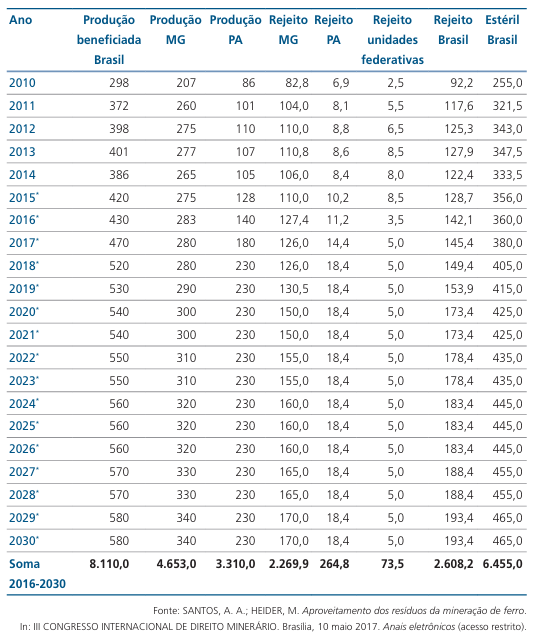
\includegraphics[width=0.9\textwidth]{figures/image17_producao_minerio.png}
    \caption{Produção beneficiada de minério de ferro, volume de rejeito e de estéril (milhões de t).}
    \label{fig:producao_minerio}
    \fonte{\citeauthor{carvalho2018} (\citeyear{carvalho2018})}
\end{figure}

Entre os minerais não metálicos, os agregados para construção civil, como brita, cascalho, areia e calcário são consumidos quase em seu estado bruto, já a produção de minério de ferro requer processos de concentração. Esses processos fazem com que o minério de ferro gere o maior volume de rejeitos minerais no país \cite{carvalho2018}.

A razão para essa associação significativa entre a produção dos principais minerais metálicos no Brasil e a geração de resíduos é que a produção dos minerais metálicos, ao contrário de alguns não metálicos que podem ser usados com mínimo beneficiamento, requer processos intensos de beneficiamento (tratamento). É esse processo de beneficiamento que gera a maior quantidade de rejeitos. Por exemplo, no caso do minério de ferro, o teor médio de ferro contido no minério beneficiado é de 63,72\%, sendo o restante do material resultante geralmente sem valor comercial, conhecido como rejeito. Os rejeitos de minério de ferro representam 35\% do volume total armazenado em barragens no Brasil, segundo dados de 2018 \cite{ibram2016, freire2020}; compondo 36,30\% das barragens incluídas na Política Nacional de Segurança de Barragens em 2015 \cite{carvalho2018}.

A vasta produção anual brasileira de ferro resulta, portanto, em um grande volume de rejeitos de minério de ferro. A Vale S/A, a maior mineradora brasileira, produziu 320 milhões de toneladas apenas de minério de ferro em 2022 \cite{pmb2023}. O aumento da demanda por insumos minerais e a viabilidade de lavrar minérios com teores mais baixos nos últimos anos também contribuíram para um crescimento igualmente crescente na geração de resíduos da mineração \cite{ibram2016}.

A mineração, e consequentemente a geração de resíduos, está prevista na Política Nacional de Resíduos Sólidos (PNRS - Lei 12.305/2010), sendo os resíduos de mineração uma das categorias de resíduos sólidos abrangidas pela lei \cite{freire2020}.

Portanto, a produção em alta escala dos principais minerais metálicos, impulsionada pelo minério de ferro, demanda processos de beneficiamento que, por sua natureza, resultam na geração de grandes volumes de resíduos (estéril da extração e rejeito do beneficiamento), tornando a gestão desses materiais um aspecto crucial e desafiador da atividade mineradora no Brasil \cite{freire2020}.

\subsubsection{Gestão de resíduos e métodos de disposição de rejeitos}

A atividade minerária, desde suas origens históricas com métodos rudimentares, tem enfrentado o desafio intrínseco da gestão dos resíduos gerados, principalmente os rejeitos provenientes do processo de beneficiamento do minério. A extração e o tratamento mineral implicam na movimentação de volumes massivos de material, dos quais apenas uma fração é a substância mineral útil, gerando um grande volume de materiais sem valor econômico imediato que requerem destinação adequada \cite{freire2020}. A disposição desses rejeitos, que frequentemente se apresentam misturados à água \cite{lozano2006}, é um desafio significativo na mineração e exige a seleção de métodos adequados \cite{cardozo2017}.

Os métodos para a disposição dos rejeitos podem ser categorizados principalmente em três formas: a céu aberto, subterrânea e subaquática. A disposição a céu aberto é a modalidade mais comum e amplamente utilizada, ocorrendo geralmente em pilhas controladas ou em estruturas de contenção, como barragens de rejeitos, localizadas em bacias ou vales que requerem barreiras. Alternativamente, a disposição subterrânea é realizada preenchendo câmaras que sobram após a extração do minério, para onde os rejeitos são bombeados. Já a disposição subaquática não é frequentemente empregada devido aos impactos negativos, muitas vezes irreversíveis, que gera nos ecossistemas aquáticos \cite{lozano2006}.

Dentre as formas de disposição a céu aberto, as barragens de rejeitos são estruturas de contenção de rejeitos e água oriundos do beneficiamento de minério \cite{lozano2006}, e são o método mais comum de disposição de rejeitos no Brasil \cite{ibram2016}.

A construção dessas estruturas é realizada em etapas sucessivas (alteamentos) utilizando diferentes metodologias, sendo as três principais: método a montante, método a jusante e método de linha de centro \cite{ibram2006}. O método a montante, por ser considerado o mais antigo, simples e econômico, tornou-se amplamente empregado na mineração brasileira. A escolha entre esses métodos de alteamento impacta diretamente a segurança, o custo e a viabilidade da estrutura ao longo de sua vida útil \cite{cardozo2017}. Além desses métodos tradicionais, outras tecnologias de disposição a céu aberto incluem pilhas controladas e o preenchimento de cavas exauridas, além de métodos que visam reduzir o teor de água dos rejeitos para empilhamento, como o empilhamento drenado ou "pervious dam" e o empilhamento a seco ("dry stacking") \cite{ibram2016}.

Diante dos riscos e impactos associados às barragens de rejeitos, especialmente após acidentes graves, novas abordagens para a destinação desses materiais ganharam destaque \cite{freire2020}. Uma importante rota é a recuperação e reaproveitamento dos rejeitos, considerando que o rejeito de hoje pode se tornar o minério de amanhã. A busca por alternativas tecnológicas sem barragens e o desenvolvimento de tecnologia para o aproveitamento econômico desses materiais têm sido recomendados \cite{carvalho2018}.

O aproveitamento de rejeitos exige rigorosa caracterização técnica para garantir que sua reutilização não transfira problemas ambientais ou técnicos para outros setores. Normas técnicas brasileiras estabelecem procedimentos para amostragem (NBR 10007) e classificação ambiental de resíduos (NBR 10004), com ensaios de lixiviação e solubilização (NBR 10005, NBR 10006). A granulometria e propriedades químicas, que variam conforme o mineral e o beneficiamento, são fatores cruciais. Estudos sobre rejeitos de minério de ferro são particularmente relevantes pela sua importância econômica e volume gerado \cite{freire2020}.

Pesquisas têm demonstrado a viabilidade técnica do uso de rejeitos de minério de ferro na construção civil, como agregado em microrrevestimento asfáltico, em argamassas substituindo areia ou cimento, e na produção de blocos de concreto intertravados com resultados mecânicos promissores. Além do desempenho técnico, o rejeito de ferro pode conferir estética avermelhada às peças \cite{freire2020}. Além disso, alguns novos projetos de mineração já incluem, desde o início, a preocupação ambiental e utilizam métodos como filtragem e empilhamento a seco para a disposição de rejeitos, evitando barragens. Há também foco na recuperação de partículas finas e grossas por flotação para melhor aproveitamento do recurso mineral e diminuição do material a ser depositado em barragens \cite{pmb2023}. Estes exemplos ilustram o potencial de valorização dos rejeitos, representando o próximo estágio para uma mineração sustentável no Brasil. A continuidade em pesquisa, regulamentação clara e fiscalização eficaz são indispensáveis para transformar os rejeitos de um passivo em um recurso \cite{ibramlivroverde2022}.

A determinação do método de disposição de rejeito mais adequado para um empreendimento mineral é um processo complexo que exige a análise de múltiplos fatores, indo além da simples escolha entre barragens ou outros sistemas \cite{lozano2006}. Fatores como a natureza do processo de mineração, as condições geológicas e topográficas da região, as propriedades mecânicas dos materiais de rejeito e estéril, a presença de contaminantes perigosos nos rejeitos e as condições climáticas locais são essenciais \cite{ibram2016}. O planejamento rigoroso e a análise multicriterial, juntamente com a experiência dos profissionais e a consideração dos custos para minimizar riscos versus custos de acidentes, são fundamentais para uma decisão assertiva \cite{lozano2006}.

\subsection{Tipos de barragens de rejeitos}
\label{subsec:tipos_barragens}

Barragens de rejeitos constituem estruturas de engenharia essenciais para a indústria mineral, servindo como depósitos para os materiais residuais gerados durante o beneficiamento do minério. Estas obras são projetadas para reter o volume de sólidos e a água remanescente dos processos industriais, que são compostos por lama, areia e água \cite{lozano2006, warzynski2023}. A função primordial dessas estruturas é confinar os rejeitos de forma segura, prevenindo sua dispersão descontrolada no ambiente e mitigando os significativos impactos negativos associados a vazamentos ou rupturas \cite{warzynski2023}.

De acordo com a NBR 13028/2017, as barragens de mineração são definidas como:

\begin{quote}
Barragens, barramentos, diques, reservatórios, cavas exauridas com barramentos construídos, associados às atividades desenvolvidas com base em direito minerário, utilizados para fins de contenção, acumulação ou decantação de rejeito de mineração ou descarga de sedimentos provenientes de atividades em mineração, com ou sem captação de água associada, compreendendo a estrutura do barramento e suas estruturas associadas. \cite{abnt2017}
\end{quote}

Historicamente, a forma de lidar com os rejeitos minerais passou por uma evolução, desde práticas rudimentares até a adoção de técnicas de contenção mais sofisticadas. Até o século XV, a geração de rejeitos pela mineração e seus impactos ambientais eram considerados insignificantes \cite{desouzajunior2018, freire2020}. Contudo, com o advento da força a vapor e o substancial aumento na capacidade de processamento de minerais, o volume de rejeitos cresceu exponencialmente, levando à busca por métodos de disposição, com as barragens de contenção emergindo como a técnica mais comumente adotada por mineradoras e profissionais de geotecnia \cite{desouzajunior2018}.

O planejamento e a concepção dessas barragens requerem um conhecimento profundo das características dos materiais envolvidos e do meio físico, iniciando-se idealmente com a seleção de um local adequado, considerando uma ampla gama de variáveis, incluindo aspectos geológicos, hidrológicos, geotécnicos, ambientais e de risco. A forma como essas estruturas são projetadas e construídas, incluindo os métodos de alteamento utilizados para aumentar sua capacidade ao longo do tempo, tem um impacto direto em sua estabilidade e segurança operacional \cite{lozano2006}.

\subsubsection{Métodos de Alteamento de Barragens de Contenção de Rejeitos}

A necessidade crescente de dispor grandes volumes de rejeitos de forma segura impulsionou o desenvolvimento de distintos métodos construtivos para as barragens. Do ponto de vista da engenharia geotécnica e das práticas convencionais, a literatura descreve três métodos principais de construção e alteamento para barragens de rejeitos. Estes métodos são denominados alteamento a montante, alteamento a jusante e alteamento pela linha de centro, refletindo a direção do deslocamento do eixo da barragem à medida que sua altura é aumentada \cite{soares2010}.

Segundo \citeonline{warzynski2023}, as barragens de rejeitos são estruturas utilizadas na indústria de mineração para armazenar os resíduos resultantes do processo de extração e beneficiamento do minério. Elas têm como objetivo conter os rejeitos, compostos por lama, areia e água, evitando sua dispersão no ambiente e os impactos negativos associados.

A escolha entre estes métodos é influenciada por uma complexa interação de fatores, tais como as características topográficas do local de implantação, o regime hidrológico, a geologia e as propriedades geotécnicas do subsolo, as características específicas dos rejeitos (granulometria, concentração), a taxa de deposição, a variação da capacidade de armazenamento e a disponibilidade de equipamentos e materiais. Entender as particularidades de cada método é fundamental para avaliar a segurança e a viabilidade de uma barragem de rejeitos específica \cite{soares2010, warzynski2023}.

\subsubsubsection{Método de Alteamento a Montante}

O método de alteamento a montante (Figura \ref{fig:metodo_montante}) é frequentemente citado como o mais antigo, simples e, historicamente, o mais econômico em termos de custos iniciais, podendo ser até 70\% mais barato que alternativas \cite{ibram2016, thome2018}. Este método começa com a construção de um dique de partida, geralmente feito de material argiloso ou enrocamento (blocos de pedra) compactado. Subsequentemente, os rejeitos são lançados a partir da crista desse dique inicial, formando uma "praia" a montante que, após adensamento, serve de fundação para os alteamentos futuros, os quais são construídos com o próprio material mais grosso dos rejeitos segregados \cite{ibram2016, carvalho2018}. 

\begin{figure}[!htb]
    \centering
    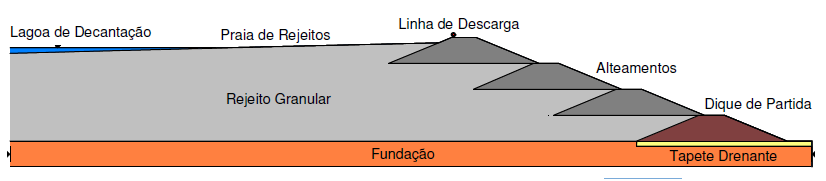
\includegraphics[width=0.9\textwidth]{figures/image18_metodo_montante.png}
    \caption{Seção típica de uma barragem alteada para montante.}
    \label{fig:metodo_montante}
    \fonte{\citeauthor{albuquerque2004} (\citeyear{albuquerque2004})}
\end{figure}

No entanto, essa prática de construir sobre rejeito previamente depositado, que ainda pode estar em processo de adensamento ou saturado, torna o método a montante altamente suscetível a problemas de estabilidade, incluindo escorregamentos e potencial de liquefação \cite{araujo2006}. Embora econômico, o método a montante apresenta desafios técnicos significativos que têm sido associados a um maior risco de ruptura \cite{thome2018}.

Conforme destaca \citeonline{araujo2006}, o método de alteamento a montante, apesar de ser amplamente adotado pela indústria mineradora, apresenta graves deficiências quanto à segurança estrutural. Sua principal vulnerabilidade reside na prática de realizar alteamentos sucessivos sobre rejeitos não consolidados, os quais, em condições de saturação e baixa compactação, demonstram reduzida resistência ao cisalhamento e elevada susceptibilidade à liquefação quando submetidos a carregamentos dinâmicos ou estáticos. Adicionalmente, este método construtivo impõe obstáculos significativos à implementação de sistemas de drenagem interna eficientes, comprometendo o controle do nível d'água na estrutura e, consequentemente, aumentando os riscos de instabilidade da barragem como um todo.

\begin{figure}[!htb]
    \centering
    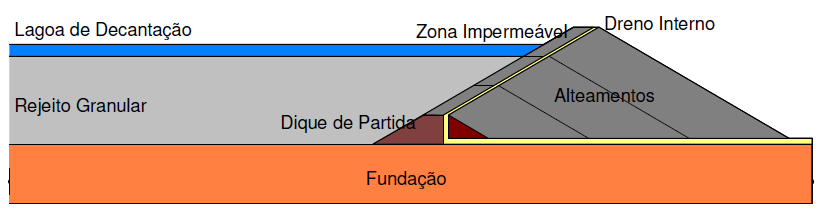
\includegraphics[width=0.9\textwidth]{figures/image19_jusante.png}
    \caption{Seção de um alteamento para montante sobre barragem existente.}
    \label{fig:metodo_montante_barragem_existente}
    \fonte{\citeauthor{albuquerque2004} (\citeyear{albuquerque2004})}
\end{figure}

\subsubsubsection{Método de Alteamento a Jusante}

Em contraste com o método a montante, o alteamento a jusante (Figura \ref{fig:metodo_jusante}) é amplamente reconhecido por sua maior segurança intrínseca, decorrente principalmente do controle construtivo e do fato de os alteamentos não serem realizados sobre a massa de rejeitos previamente depositada, embora geralmente associado a custos mais elevados. Neste método, o dique de partida, construído com materiais convencionais como solo ou enrocamento compactado, serve de base, e os alteamentos subsequentes são edificados integralmente para jusante, distanciando-se do reservatório de rejeitos, expandindo a barragem para fora \cite{ibram2016, ctsufsj2017}.

\begin{figure}[!htb]
    \centering
    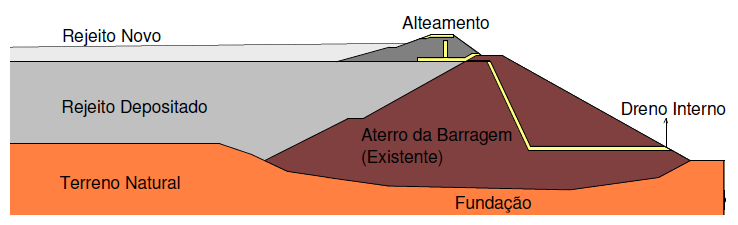
\includegraphics[width=0.9\textwidth]{figures/image18_montante_cont.png}
    \caption{Seção típica de uma barragem alteada para jusante.}
    \label{fig:metodo_jusante}
    \fonte{\citeauthor{albuquerque2004} (\citeyear{albuquerque2004})}
\end{figure}

As vantagens do método a jusante incluem a possibilidade de maior controle sobre a compactação dos materiais constituintes e a facilidade de instalação e extensão de sistemas de drenagem interna durante a construção, o que permite um controle mais eficaz da linha freática dentro do maciço da barragem, aumentando sua estabilidade. Barragens construídas a jusante geralmente requerem um maior volume de material de construção, especialmente a fração mais grossa (areia) obtida por ciclonagem. Apesar do custo potencialmente mais alto, a capacidade de projetar e construir a estrutura com a resistência necessária desde o início, inclusive para resistir a eventos sísmicos, faz deste método uma opção tecnicamente mais robusta \cite{araujo2006, ibram2016}.

\subsubsubsection{Método de Alteamento pela Linha de Centro}

Situado como uma alternativa intermediária em termos de custo e risco entre os métodos a montante e a jusante, encontra-se o alteamento pela linha de centro (Figura \ref{fig:metodo_linha_de_centro}). Este método começa com um dique de partida, e os alteamentos subsequentes são construídos de forma que o eixo da crista da barragem permaneça aproximadamente na mesma posição horizontal (linha de centro) enquanto a altura da estrutura aumenta. O crescimento ocorre tanto verticalmente quanto ligeiramente para fora, sobre a linha de centro ou sutilmente a jusante \cite{soares2010, ctsufsj2017}.

\begin{figure}[!htb]
    \centering
    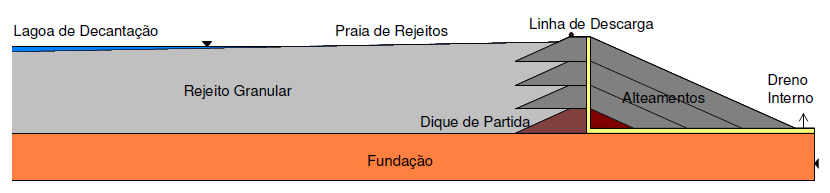
\includegraphics[width=0.9\textwidth]{figures/image20_linha_de_centro.png}
    \caption{Seção típica de uma barragem alteada pela linha de centro.}
    \label{fig:metodo_linha_de_centro}
    \fonte{\citeauthor{albuquerque2004} (\citeyear{albuquerque2004})}
\end{figure}

Embora apresente um risco inferior ao método a montante por não avançar continuamente sobre o rejeito saturado mais mole, pode ainda envolver a construção de diques sobre rejeitos parcialmente consolidados na área da linha de centro, o que o torna potencialmente menos seguro que o alteamento a jusante \cite{duarte2008}.

Neste caso, a construção dos alteamentos ocorre a partir de um eixo central, com os alteamentos subsequentes avançando para jusante, mas de forma que a crista da barragem se mantenha aproximadamente na mesma posição horizontal inicial. A fundação dos alteamentos repousa parcialmente sobre a "praia" de rejeitos já depositados, e parcialmente sobre o dique original ou materiais de empréstimo \cite{ibram2016}. Barragens construídas por este método recebem uma classificação de risco intermediária em alguns sistemas de avaliação \cite{duarte2008}.

A escolha do método a ser utilizado depende de diversos fatores, como o tipo de rejeito, área disponibilizada e abalos sísmicos. Dessa maneira, a Tabela~\ref{tab:caracteristicas_barragens} mostra um comparativo entre esses três métodos, evidenciando suas características distintas; e a Tabela~\ref{tab:vantagens_desvantagens} mostra as vantagens e desvantagens dos três tipos de barragens de rejeitos.

% Tabela 1: Características dos Métodos Construtivos de Barragens de Rejeitos
\begin{table}[h!]
    \centering
    \caption{Características dos principais métodos construtivos de barragens de rejeitos}
    \label{tab:caracteristicas_barragens}
    \begin{tabular}{|p{3.8cm}|p{3.3cm}|p{3.3cm}|p{3.3cm}|}
        \hline
        \textbf{Características} & 
        \textbf{Montante} & 
        \textbf{Jusante} & 
        \textbf{Linha de Centro} \\
        \hline
        \textbf{Tipo de rejeito recomendado} & 
        Baixa densidade para que ocorra segregação. Mais de 40\% de areia & 
        Qualquer tipo & 
        Áreas ou lamas de baixa plasticidade \\
        \hline
        \textbf{Descarga de rejeitos} & 
        Periférica & 
        Independe. De acordo com o projeto & 
        Periférica, conservando o eixo da barragem \\
        \hline
        \textbf{Armazenamento de água} & 
        Não recomendável para grandes volumes & 
        Bom & 
        Aceitável. Não recomendado para armazenamento permanente \\
        \hline
        \textbf{Resistência sísmica} & 
        Baixa. Fraca em áreas de alta sismicidade & 
        Boa & 
        Aceitável \\
        \hline
        \textbf{Alteamentos} & 
        Ideal menos 10~m/ano. Recomendável menos de 5 a 10~m/ano, perigoso mais alto que 15~m/ano & 
        Nenhuma restrição & 
        Pouca restrição \\
        \hline
        \textbf{Requisitos de alteamento} & 
        Solo natural e/ou rejeitos ou estéril & 
        Rejeitos ou estéril & 
        Rejeitos ou estéril \\
        \hline
        \textbf{Custo relativo do corpo do aterro} & 
        Baixo $V_m$. Menor custo, utilizado onde há restrição de área & 
        Alto (3 $V_m$). Grande quantidade de material requerido & 
        Moderado (2 $V_m$). Flexibilidade construtiva \\
        \hline
    \end{tabular}
    \footnotesize
    Fonte: Adaptado de \citeauthor{freire2020} (\citeyear{freire2020}) (pag. 111) e \citeauthor{lozano2006} (\citeyear{lozano2006}) (pag. 29).
\end{table}

% Tabela 2: Vantagens e Desvantagens dos Métodos Construtivos
\begin{table}[h!]
    \centering
    \caption{Vantagens e desvantagens dos três tipos de barragens de rejeitos}
    \label{tab:vantagens_desvantagens}
    \begin{tabular}{|p{2.3cm}|p{3.8cm}|p{3.8cm}|p{3.8cm}|}
        \hline
         & 
        \textbf{Método de Montante} & 
        \textbf{Método de Jusante} & 
        \textbf{Método da Linha de Centro} \\
        \hline
        \textbf{Método construtivo} & 
        Método mais antigo, e o mais empregado. Construção de dique inicial e os diques do alteamento periféricos com material de empréstimo, estéreis da lavra ou com ``underflow'' de ciclonagem. Lançamento a partir da crista por ciclonagem ou ``spigots''. & 
        Construção de dique inicial impermeável e barragem de pé. Separação dos rejeitos na crista do dique por meio de hidrociclones. Dreno interno e impermeabilização a montante. & 
        Variação do método de jusante. \\
        \hline
        \textbf{Vantagens} & 
        Menor custo. Maior velocidade de alteamento. Utilizado em lugares onde há limitante de área. & 
        Maior segurança. Compactação de todo o corpo da barragem. Pode-se misturar os estéreis da lavra. & 
        Variação do volume de ``underflow'' necessário com relação ao método da jusante. \\
        \hline
        \textbf{Desvantagens} & 
        Baixa segurança devido à linha freática próxima ao talude de jusante, susceptibilidade de liquefação, possibilidade de ``piping''. & 
        Necessidade de grandes quantidades de ``underflow'' (problemas nas 1\textsuperscript{as} etapas). Deslocamento do talude de jusante (proteção superficial só no final da construção). & 
        Necessidade de sistemas de drenagem eficientes e sistemas de contenção a jusante. \\
        \hline
    \end{tabular}
    \footnotesize
    Fonte: Adaptado de \citeauthor{lozano2006} (\citeyear{lozano2006}) (pag. 29).
\end{table}

% Nota: $V_m$ = volume da barragem alteada pelo método de montante

Além dos três modelos construtivos citados anteriormente, existe o método ``Etapa Única'' (Single Stage), no qual não há alteamentos após a construção inicial. Neste sistema, a barragem é construída em solo compactado ou enrocamento, até a sua altura final em uma única etapa, sendo mais comumente utilizado para instalações de rejeitos menores. Este método difere fundamentalmente dos demais por não permitir expansões futuras da capacidade de armazenamento, exigindo dimensionamento preciso desde a fase inicial do projeto \cite{vale2024, teck2019}.

Segundo consulta realizada no Sistema Integrado de Gestão de Barragens de Mineração (SIGBM) em maio de 2025, conforme mostra a Figura~\ref{fig:distribuicao_barragens}, a distribuição das barragens por método construtivo revela uma predominância significativa da construção em etapa única, representando 492 estruturas (53,9\% do total cadastrado). O método de alteamento a jusante aparece como a segunda opção mais utilizada, com 217 barragens (23,8\%), seguido pelo alteamento por linha de centro com 113 estruturas (12,4\%). Em contraste, o método de alteamento a montante, reconhecido pela literatura técnica como potencialmente mais vulnerável, corresponde a apenas 51 barragens (5,6\% do total). Observa-se ainda a existência de 38 barragens classificadas como ``indefinido'' (4,2\%) e 7 como ``desconhecido'' (0,8\%), indicando a necessidade de complementação de informações técnicas para essas estruturas \cite{anmsistema2020}.

\begin{figure}[!htb]
    \centering
    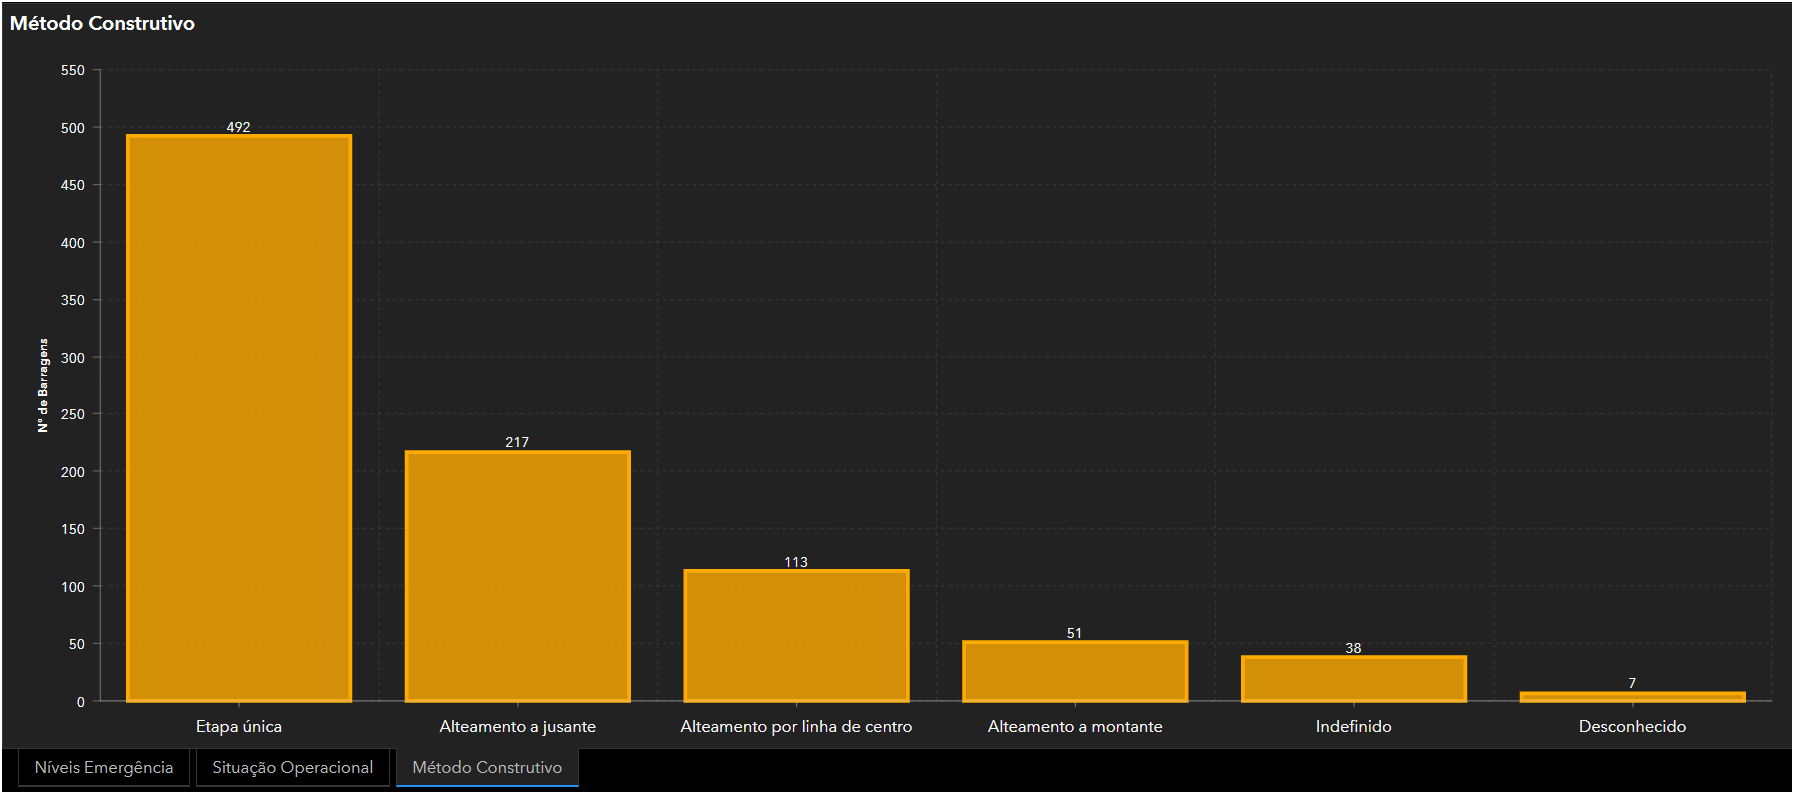
\includegraphics[width=0.9\textwidth]{figures/image21_distribuicao_barragens_por_metodo_atual.png}
    \caption{Distribuição das barragens por método construtivo}
    \label{fig:distribuicao_barragens}
    \fonte{\citeauthor{anmsistema2020} (\citeyear{anmsistema2020})}
\end{figure}

Em suma, enquanto o método a montante oferece vantagens econômicas iniciais notáveis, o método a jusante é tecnicamente mais robusto e seguro, especialmente em termos de estabilidade e controle de percolação, embora apresente um custo mais elevado \cite{desouzajunior2018}. Por sua vez, o método pela linha de centro busca um equilíbrio, combinando aspectos dos outros dois, e seu comportamento geotécnico se aproxima mais do método a jusante. Portanto, a análise comparativa desses métodos é fundamental para orientar a tomada de decisão técnica mais adequada a cada contexto específico \cite{araujo2006}.

A segurança e a gestão de barragens de rejeitos ganharam foco global e nacional após acidentes catastróficos, como os de Mariana (2015) e Brumadinho (2019) no Brasil, que foram associados a barragens com alteamento a montante. Estes eventos trágicos evidenciaram a necessidade urgente de revisão e fortalecimento das regulamentações e padrões de segurança \cite{warzynski2023}. A legislação brasileira, por exemplo, foi atualizada, com a NBR 13028 (2017) estabelecendo requisitos mínimos para projetos, incorporando critérios mais rigorosos para fatores de segurança, análises de risco, estudos tecnológicos e sísmicos, e a obrigatoriedade de Planos de Ações Emergenciais (PAE) para barragens com alto Dano Potencial Associado (DPA) \cite{desouzaaraujo2018}. De acordo com a Lei nº 12.334/2010, é obrigatório ``exigir do empreendedor a anotação de responsabilidade técnica, por profissional habilitado pelo Sistema Conselho Federal de Engenharia e Agronomia (Confea) / Conselho Regional de Engenharia e Agronomia (Crea), bem como o cumprimento das recomendações presentes nos relatórios de inspeção e revisão de segurança'' \cite{brasil2010pnsb}.

Em Minas Gerais, berço de grande parte desses acidentes, o Decreto estadual 46.993/2016, fundamentado nas características técnicas e na maior suscetibilidade do método a montante, instituiu medidas mais rigorosas e suspendeu o licenciamento ambiental para novas barragens que utilizassem essa técnica. Essas mudanças regulatórias refletem uma clara tendência para desencorajar ou proibir os métodos de disposição considerados de maior risco \cite{ibram2016, thome2018}.

"Em relação ao dano potencial associado (DPA) pode-se afirmar que representa uma avaliação que relaciona entre o volume de rejeitos no reservatório e os impactos sociais, ambientais e econômico." \cite{desouzajunior2018}

A avaliação contínua da segurança estrutural e ambiental das barragens é garantida, em grande parte, pela implementação e monitoramento de sistemas de instrumentação. Estes sistemas são projetados para medir parâmetros geotécnicos e ambientais cruciais que indicam o comportamento da estrutura ao longo do tempo \cite{soares2010}. Instrumentos como piezômetros (do tipo ``Stand pipe'' ou elétricos de corda vibrante) monitoram os níveis de água no interior da barragem, placas de recalque e marcos de deslocamentos superficiais medem deformações, e medidores de vazão controlam a percolação. O acompanhamento desses dados, idealmente com frequência regular (semanal ou quinzenal, ou diária em situações críticas), permite identificar anomalias e tomar medidas corretivas em tempo hábil para manter a segurança \cite{soares2010, desouzajunior2018}.

Complementar à instrumentação e ao monitoramento de campo, a análise de estabilidade, frequentemente realizada com o auxílio de ferramentas de modelagem numérica, é fundamental nas fases de projeto e operação. A avaliação da estabilidade de barragens de rejeitos, conforme diretrizes normativas como a NBR 13028 \cite{abnt2017}, exige análises rigorosas do maciço, da fundação e das interações entre eles. Essas análises abrangem o dique de partida, a fundação, os alteamentos e o próprio corpo de rejeito, visando identificar superfícies potenciais de ruptura. A modelagem numérica, particularmente utilizando o Método de Elementos Finitos (MEF), tornou-se uma ferramenta padrão para simular o comportamento tensão-deformação da estrutura, prevendo recalques, deformações e potenciais zonas de ruptura \cite{desouzajunior2018}. 

A análise de percolação também é vital para entender o fluxo de água dentro e sob a barragem, utilizando redes de fluxo para estimar poropressões que influenciam a estabilidade em condições drenadas. A contínua pesquisa e aplicação dessas técnicas são cruciais para aprimorar tanto os projetos de barragens quanto as soluções de disposição alternativas. Projetistas utilizam rotineiramente softwares comerciais que implementam métodos de equilíbrio limite para realizar essas verificações, como os métodos de Bishop simplificado, Janbu, Spencer, e Morgenstern \& Price \cite{araujo2006, desouzajunior2018}.

A análise dos acidentes históricos e a literatura especializada sobre falhas em barragens de rejeitos indicam que, embora as causas técnicas (como liquefação e entubamento) sejam bem definidas, a origem primária dos problemas frequentemente reside em falhas de gestão. As principais causas de acidentes são atribuídas à liquefação (46,7\%) e ao entubamento (24,4\%) \cite{soares2010}. No entanto, o gerenciamento inadequado ou a má execução de projetos e administração são vistos como os fatores que permitem que as condições técnicas desfavoráveis se desenvolvam e levem à ruptura \cite{duarte2008, carneiro2018}.

A evolução das normas, a busca por métodos construtivos mais seguros e a crescente exploração do reaproveitamento de rejeitos refletem uma maior maturidade do setor mineral em relação aos desafios ambientais e de segurança. O setor reconhece a necessidade de aprender com os acidentes e aprimorar suas práticas de gestão. A preocupação com o meio ambiente transcendeu a teoria e se manifesta em ações para reduzir impactos. Apesar dos avanços, persistem desafios como a complexidade regulatória e a necessidade de formar profissionais qualificados \cite{pmb2023}.

\subsection{Panorama Brasil vs. Mundo}

A implementação de diferentes metodologias construtivas para barragens de contenção de rejeitos constitui uma prática amplamente difundida no cenário minerário internacional, incluindo o contexto brasileiro, onde é adotada sistematicamente por empresas de grande porte do setor. A Vale S.A., uma das maiores corporações mineradoras globais, emprega estrategicamente os métodos de alteamento a jusante, a montante e por linha de centro em suas diversas operações, adaptando a escolha técnica às características geotécnicas específicas de cada empreendimento \cite{vale2024}. Similarmente, a Teck Resources Limited diversifica sua abordagem construtiva, utilizando os métodos upstream (a montante), downstream (a jusante), centreline (linha de centro) e single stage (etapa única), além de combinações híbridas desses sistemas, distribuídos entre suas unidades operacionais no Canadá, Estados Unidos e Chile, demonstrando a versatilidade e adaptabilidade regional dessas tecnologias \cite{teck2019}.

Contudo, a análise crítica dos métodos revela disparidades significativas em termos de desempenho técnico e segurança operacional. O método de alteamento a montante, apesar de apresentar vantagens econômicas substanciais que o tornam amplamente adotado na mineração brasileira devido aos menores custos de implementação e menor demanda de materiais de construção, manifesta limitações estruturais consideráveis. Estas limitações se traduzem em menor confiabilidade geotécnica, maior suscetibilidade a instabilidades e elevada propensão a falhas catastróficas, particularmente quando submetido a condições adversas como eventos sísmicos, variações do nível freático ou saturação excessiva dos materiais depositados \cite{cardozo2017}.

O método de alteamento a montante tem enfrentado crescentes restrições em diversos países devido às suas vulnerabilidades estruturais intrínsecas. Segundo \cite{thome2018}, esta técnica construtiva tornou-se proibida em algumas jurisdições internacionais, particularmente em regiões geologicamente instáveis. O Chile e o Peru, países situados na zona de convergência das placas tectônicas de Nazca e Sul-Americana, exemplificam essa tendência restritiva ao não admitirem a aplicação dessa metodologia em seus territórios. A decisão técnica desses países fundamenta-se na incompatibilidade entre o método a montante e as condições sísmicas características dessas regiões, onde a atividade tectônica intensa gera tremores de terra que podem comprometer severamente a estabilidade estrutural das barragens construídas por essa técnica.

No contexto brasileiro, a regulamentação do método a montante evoluiu gradualmente, inicialmente através de medidas de controle e auditoria. O Decreto n. 46.993, de 2 de maio de 2016, do Estado de Minas Gerais, representou um marco inicial ao instituir a Auditoria Técnica Extraordinária de Segurança de Barragem especificamente para empreendimentos que utilizassem ou tivessem utilizado o método de alteamento a montante para disposição de rejeitos de mineração. Esta medida reconhecia implicitamente os riscos associados a essa metodologia construtiva, estabelecendo mecanismos de monitoramento mais rigorosos para estruturas consideradas menos seguras em relação aos demais métodos disponíveis \cite{thome2018}.

A legislação brasileira experimentou uma transformação radical em 2019, quando foi estabelecida a proibição completa da construção e alteamento de barragens de mineração pelo método a montante. Esta decisão legislativa foi diretamente motivada pelos desastres ambientais de proporções catastróficas ocorridos em Mariana (2015) e Brumadinho (2019), considerados os maiores acidentes ambientais da história do país \cite{anm2023barragens, cbhsf2020, agenciabrasil2019}. A Lei nº 14.066/2020, que alterou substancialmente a Política Nacional de Segurança de Barragens (Lei nº 12.334/2010), formalizou essa proibição através de seu artigo 2º-A, estabelecendo de forma inequívoca que "fica proibida a construção ou o alteamento de barragem de mineração pelo método a montante" \cite{anm2023barragens, cbhsf2020}. A definição legal caracteriza este método como aquele no qual os diques de contenção se apoiam diretamente sobre o próprio rejeito ou sedimento previamente depositado, configuração que apresenta riscos estruturais significativos \cite{anm2023barragens}.

Além da proibição de novas construções, a legislação determinou a descaracterização obrigatória das estruturas preexistentes construídas ou alteadas por esse método, processo que envolve a eliminação completa da função de barragem de rejeitos. O prazo inicial estabelecido foi de 25 de fevereiro de 2022 para conclusão da descaracterização, independentemente do volume de material armazenado. Contudo, reconhecendo a complexidade técnica e operacional envolvida nesse processo, a legislação previu a possibilidade de prorrogação do prazo pela ANM, mediante comprovação de inviabilidade técnica para execução no período determinado, desde que referendada pela autoridade licenciadora ambiental competente \cite{anm2023barragens, cbhsf2020}.

No âmbito estadual, Minas Gerais adotou uma postura ainda mais restritiva através da Lei Estadual nº 23.291/2019, estabelecendo prazo mais exíguo até 25 de fevereiro de 2021 para a descaracterização. No entanto, a complexidade técnica inerente a esses processos resultou em numerosos casos de prorrogação, formalizados mediante termos de compromisso estabelecidos com o Ministério Público, demonstrando a necessidade de equilibrar urgência regulatória com viabilidade técnica de execução \cite{feam2024}.

O sistema de fiscalização das barragens de mineração opera através de uma estrutura dual, envolvendo a ANM e os órgãos ambientais estaduais. As empresas mineradoras estão sujeitas a um conjunto rigoroso de obrigações, incluindo a notificação imediata de qualquer alteração nas condições de segurança das barragens, garantindo resposta rápida a situações de risco potencial \cite{cbhsf2020}. A documentação técnica relacionada aos processos de descaracterização deve ser elaborada por profissionais habilitados e submetida à revisão por consultoria externa especializada, assegurando independência técnica na avaliação dos projetos \cite{anm2023barragens}.

As empresas devem ainda cumprir obrigações abrangentes de transparência, segurança e acompanhamento das obras, conforme especificado nos termos de compromisso firmados com os órgãos de controle competentes \cite{feam2024}. O descumprimento dessas determinações legais pode resultar em sanções severas, incluindo embargo ou suspensão integral das atividades do complexo minerário até a regularização das não-conformidades identificadas. Este sistema de penalidades visa garantir a aderência às normas de segurança e a priorização da proteção ambiental e social sobre interesses econômicos de curto prazo \cite{anm2023barragens}.

\section{Classificação de risco das barragens de rejeitos}
\label{sec:classificacao_risco}

A gestão da segurança de barragens, especialmente aquelas destinadas à acumulação de água, disposição de rejeitos e resíduos industriais, constitui um tema de crescente relevância no Brasil, impulsionado por desafios inerentes à atividade e, notavelmente, por eventos acidentais de grande impacto \cite{carvalho2018,geoscan2020}. A mineração, por exemplo, gera volumes substanciais de resíduos sólidos, grande parte dos quais é disposta em barragens de rejeitos, demandando mecanismos aprimorados de gestão e desenvolvimento de tecnologias de baixo risco. A gestão desses resíduos envolve desde o planejamento e destinação adequada até o monitoramento contínuo das estruturas de deposição \cite{carvalho2018}. A necessidade de regulamentação robusta para garantir a segurança dessas estruturas, minimizando riscos e impactos ambientais e sociais, culminou na criação de um marco legal específico \cite{cnrh2012,carvalho2018}.

Em resposta à crescente preocupação com a segurança e após acidentes significativos, foi instituída a Política Nacional de Segurança de Barragens (\textsc{PNSB}) \cite{cnrh2012,moecke2019}. A Lei nº 12.334, de 20 de setembro de 2010, estabeleceu a \textsc{PNSB}, definindo padrões mínimos de segurança para barragens de múltiplos usos (acumulação de água, disposição de rejeitos e resíduos industriais) que possuam características como altura maior ou igual a 15 m, volume maior ou igual a 3 hm³, contenham resíduos perigosos, ou apresentem dano potencial associado médio ou alto \cite{carvalho2018,moecke2019}. O objetivo primordial da \textsc{PNSB} é reduzir a ocorrência de acidentes e suas consequências, visando à proteção da população e do meio ambiente. Este marco legal inicial criou a base para um sistema de classificação que auxiliaria na implementação de medidas de segurança adequadas \cite{moecke2019}.

Com base no que foi estabelecido pela \textsc{PNSB}, o detalhamento dos critérios de classificação foi elaborado pelo Conselho Nacional de Recursos Hídricos (\textsc{CNRH}). A Resolução \textsc{CNRH} nº 143, de 10 de julho de 2012, publicada em 04/09/2012, estabeleceu os critérios gerais para a classificação das barragens \cite{cnrh2012}. Conforme esta resolução, a classificação é realizada principalmente por três vertentes: Categoria de Risco (\textsc{CRI}), Dano Potencial Associado (\textsc{DPA}) e pelo volume do reservatório \cite{cnrh2012,moecke2019}. A classificação de barragens é uma atividade fundamental, concentrada na fase inicial da implementação da \textsc{PNSB}, permitindo que as entidades fiscalizadoras conheçam o estado das estruturas sob sua jurisdição, embora a classificação possa ser alterada ao longo dos anos \cite{moecke2019}.

A Categoria de Risco (\textsc{CRI}) é classificada como alta, média ou baixa, leva em conta aspectos da própria barragem que podem influenciar a possibilidade de ocorrência de um acidente, baseando-se na avaliação de três parâmetros principais \cite{cnrh2012,geoscan2020}:

\begin{enumerate}
    \item \textbf{Características Técnicas (CT):} Avalia aspectos estruturais e de projeto da barragem, incluindo altura, comprimento, tipo de barragem, tipo de fundação, idade da barragem e vazão de projeto.
    \item \textbf{Estado de Conservação (EC):} Considera as condições físicas atuais da estrutura, incluindo a existência de percolação, deformações, deterioração dos taludes, e existência de dispositivos de controle.
    \item \textbf{Plano de Segurança da Barragem (PSB):} Verifica a existência e conformidade da documentação de segurança, incluindo o próprio Plano de Segurança, inspeções regulares, regras operacionais e relatórios de monitoramento.
\end{enumerate}

Cada um destes parâmetros recebe uma pontuação específica de 0 a 10 com base nos dados da barragem em estudo. A soma destas pontuações determina a faixa da Categoria de Risco. Um aspecto crítico nesta metodologia é que uma pontuação $\geq$ 8 em qualquer coluna de Estado de Conservação implica automaticamente na classificação como de Alto Risco, exigindo providências imediatas pelo responsável da barragem \cite{cnrh2012}.

Enquanto a Categoria de Risco (CR) foca nas condições da barragem em si, o Dano Potencial Associado (\textsc{DPA}) olha para as potenciais consequências de uma falha \cite{cnrh2012}.

Conforme definido na legislação, o Dano Potencial Associado (\textsc{DPA}) refere-se ao impacto que pode ocorrer em caso de rompimento, vazamento, infiltração ou mau funcionamento.

\begin{quote}
``V - dano potencial associado: dano que pode ocorrer devido a rompimento, vazamento, infiltração no solo ou mau funcionamento de uma barragem, independentemente da sua probabilidade de ocorrência, podendo ser graduado de acordo com as perdas de vidas humanas e impactos sociais, econômicos e ambientais;'' \cite{cnrh2012}.
\end{quote}

A classificação quanto ao \textsc{DPA} é subdividida em alto, médio ou baixo, sendo função do potencial de perda de vidas humanas e dos impactos econômicos, sociais e ambientais decorrentes de um rompimento, além da capacidade de armazenamento do reservatório \cite{brasil2010pnsb,geoscan2020}.

O artigo 5º da legislação vigente estabelece sete critérios fundamentais para a classificação do dano potencial associado em estruturas de contenção de rejeitos minerais, organizados em uma hierarquia que prioriza a proteção da vida humana e dos recursos ambientais estratégicos \cite{brasil2010pnsb}:

\begin{enumerate}
    \item \textbf{Risco à vida humana:} presença de população a jusante com potencial de perda de vidas humanas;
    \item \textbf{Infraestrutura habitacional:} existência de unidades habitacionais ou equipamentos urbanos e comunitários;
    \item \textbf{Infraestrutura geral:} presença de sistemas de infraestrutura ou serviços essenciais;
    \item \textbf{Serviços públicos:} existência de equipamentos de serviços públicos considerados essenciais;
    \item \textbf{Patrimônio ambiental:} presença de áreas protegidas definidas na legislação ambiental;
    \item \textbf{Características dos materiais:} natureza específica dos rejeitos ou resíduos armazenados; e
    \item \textbf{Dimensão física:} volume total da estrutura de contenção.
\end{enumerate}

A determinação do Dano Potencial Associado fundamenta-se em uma análise sistemática e multidisciplinar que consolida os sete critérios legais em quatro dimensões analíticas principais, cada uma contribuindo de forma ponderada e complementar para a classificação final da estrutura \cite{brasil2010pnsb,carneiro2018,geoscan2020}:

\begin{enumerate}
    \item \textbf{Dimensão física:} volume do reservatório e características técnicas da estrutura;
    \item \textbf{Dimensão humana:} existência e densidade populacional a jusante da estrutura;
    \item \textbf{Dimensão ambiental:} impacto potencial sobre ecossistemas e áreas protegidas;
    \item \textbf{Dimensão socioeconômica:} impacto sobre infraestrutura, serviços públicos e atividades econômicas regionais.
\end{enumerate}

O processo de classificação do \textsc{DPA} utiliza uma metodologia quantitativa na qual cada um dos quatro critérios mencionados recebe uma pontuação que varia de 0 a 10, baseada nas características específicas da barragem em estudo \cite{brasil2010pnsb,carneiro2018}. É importante notar que a legislação em vigor no Brasil classifica o \textsc{DPA} como alto sempre que houver ocupação permanente na área afetada a jusante da barragem, independentemente de outras características \cite{moecke2019}. Barragens classificadas com \textsc{DPA} Alto devem sempre conter um Plano de Ação de Emergência (\textsc{PAE}) \cite{freire2020}.

A classificação das barragens pela matriz de categoria de risco (\textsc{CRI}) e dano potencial (\textsc{DPA}) associado direciona a elaboração do Plano de Segurança de Barragem (PSB) e outros documentos regulatórios, como o Plano de Ação de Emergência (\textsc{PAE}) \cite{moecke2019}.

As \autoref{fig:categoria_risco_ct}, \autoref{fig:categoria_risco_ec}, \autoref{fig:categoria_risco_ps} e \autoref{fig:dano_potencial} apresentam o sistema de classificação da Categoria de Risco (CRI) e Dano Potencial Associado (DPA) proposto pelo CNRH \cite{cnrh2012}.

\begin{figure}[htbp]
    \centering
    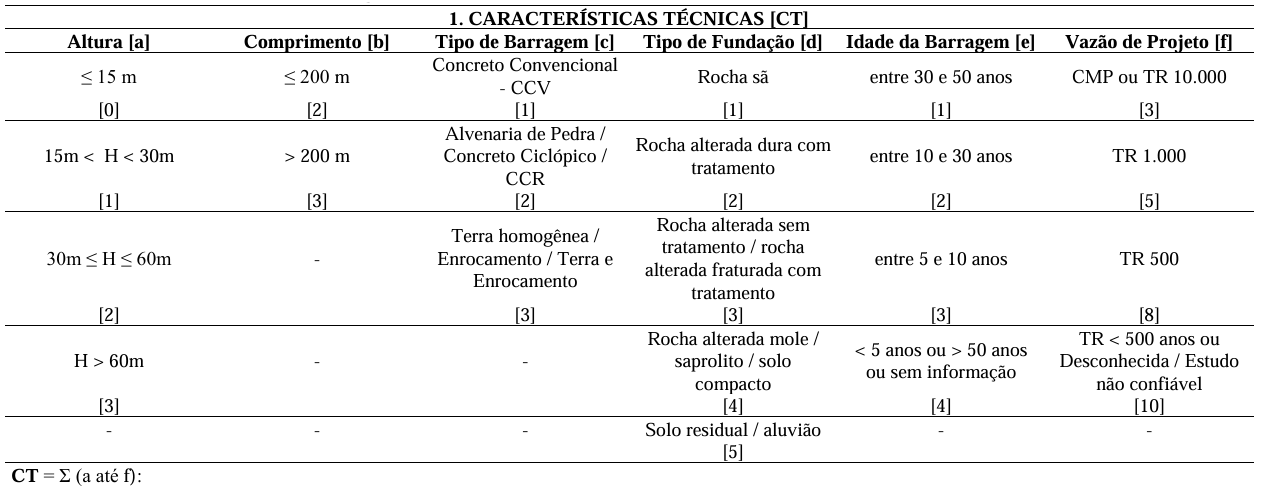
\includegraphics[width=\textwidth]{figures/image22_categoria_de_risco_ct.png}
    \caption{Matriz de classificação da Categoria de Risco (CRI) -- Características Técnicas}
    \label{fig:categoria_risco_ct}
    \fonte{\citeonline{moecke2019} de acordo com Resolução nº 143 CNRH}
\end{figure}

\begin{figure}[htbp]
    \centering
    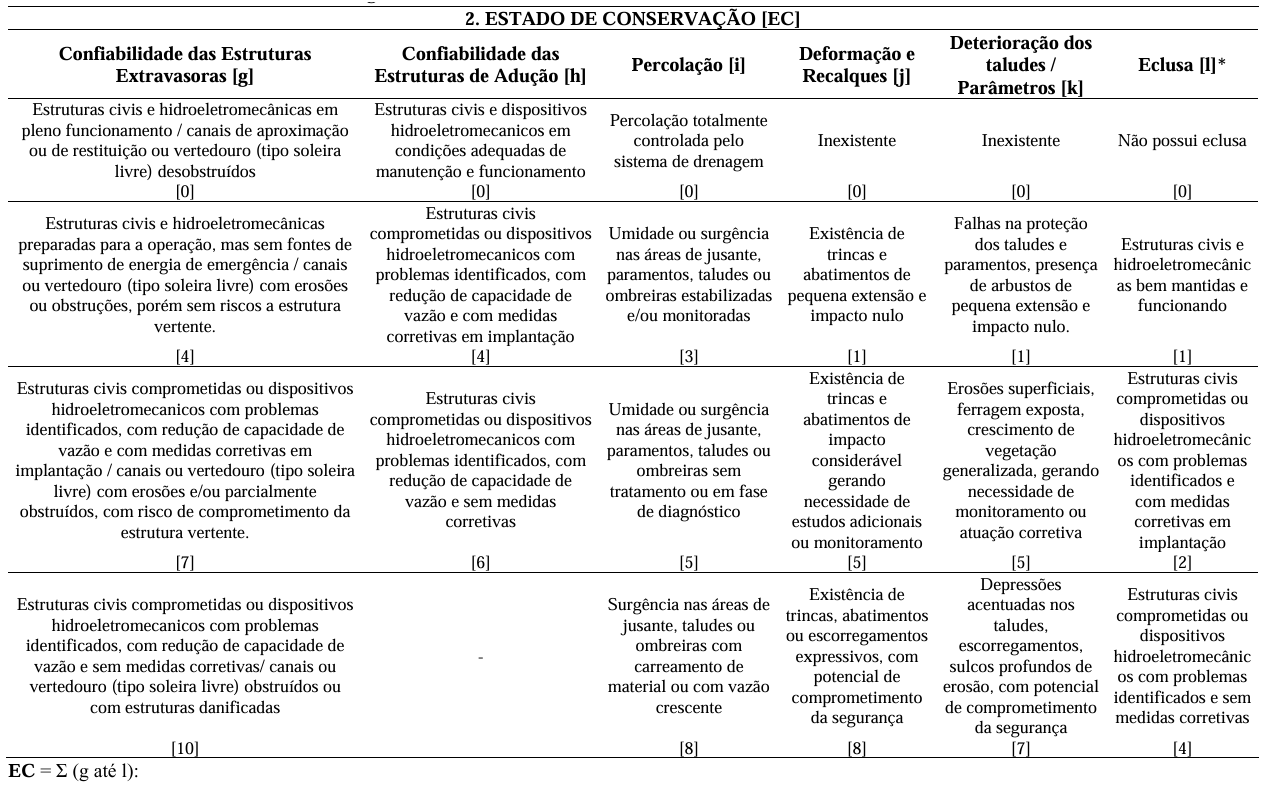
\includegraphics[width=\textwidth]{figures/image23_categoria_de_risco_ec.png}
    \caption{Matriz de classificação da Categoria de Risco (CRI) -- Estado de Conservação}
    \label{fig:categoria_risco_ec}
    \fonte{\citeonline{moecke2019} de acordo com Resolução nº 143 CNRH}
\end{figure}

\begin{figure}[htbp]
    \centering
    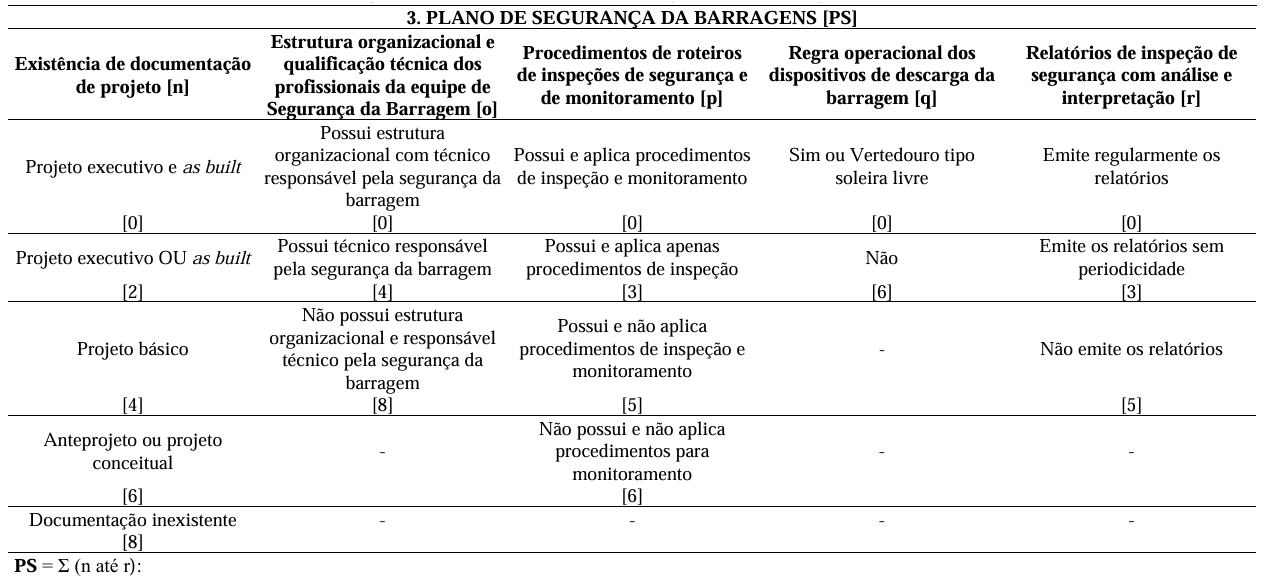
\includegraphics[width=\textwidth]{figures/image24_categoria_de_risco_ps.png}
    \caption{Matriz de classificação da Categoria de Risco (CRI) -- Plano de Segurança de Barragens}
    \label{fig:categoria_risco_ps}
    \fonte{\citeonline{moecke2019} de acordo com Resolução nº 143 CNRH}
\end{figure}

\begin{figure}[htbp]
    \centering
    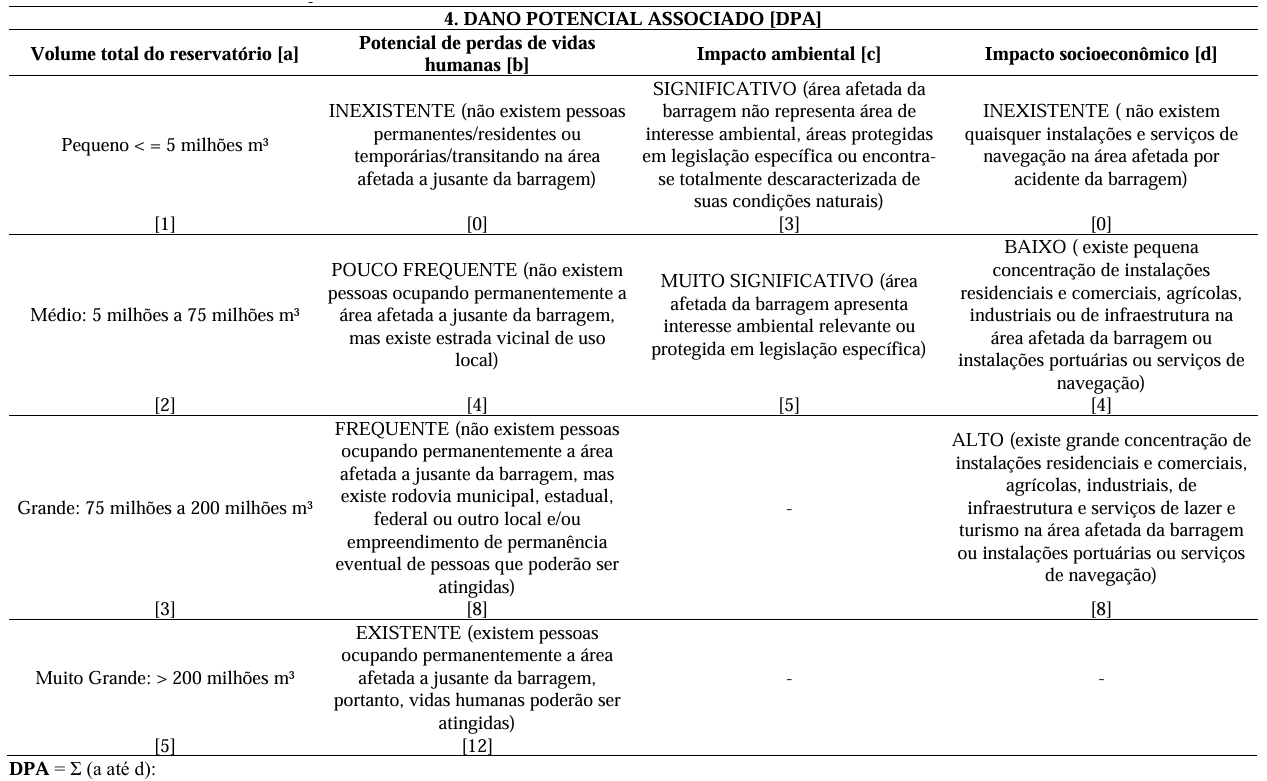
\includegraphics[width=\textwidth]{figures/image25_dano_potencial.png}
    \caption{Matriz de classificação quanto ao Dano Potencial Associado (DPA)}
    \label{fig:dano_potencial}
    \fonte{\citeonline{moecke2019} de acordo com Resolução nº 143 CNRH}
\end{figure}

O método de classificação estabelecido utiliza um total de 21 critérios técnicos, cujos valores são somados para a definição da classe de risco e de dano potencial associado \cite{cruz2024}. A metodologia segue as equações apresentadas a seguir:

\begin{equation}
\text{Classe de risco} = \sum CT + \sum EC + \sum PS
\label{eq:classe_risco}
\end{equation}

\begin{equation}
\text{Classe de dano} = \sum DPA
\label{eq:classe_dano}
\end{equation}

\noindent onde:
\begin{itemize}
    \item CT = Características Técnicas;
    \item EC = Estado de Conservação;
    \item PS = Plano de Segurança da Barragem;
    \item DPA = Dano Potencial Associado.
\end{itemize}

A partir dos valores resultantes dos somatórios, classifica-se a barragem quanto à sua categoria de risco e dano potencial associado, de acordo com a Figura~\ref{fig:matriz_cri_e_dpa} \cite{moecke2019}.

\begin{figure}[htbp]
    \centering
    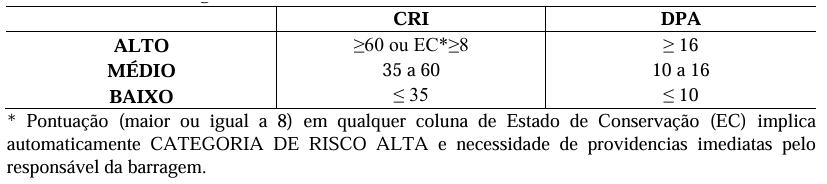
\includegraphics[width=\textwidth]{image26_matriz_cri_e_dpa.png}
    \caption{Matriz Categoria de Risco e Dano Potencial Associado}
    \label{fig:matriz_cri_e_dpa}
    \fonte{\cite{moecke2019} de acordo com Resolução nº 143 CNRH}
\end{figure}

A Resolução nº 91 da Agência Nacional de Águas (ANA), de 02 de abril de 2012, apresenta o Plano de Segurança de Barragens (PSB) como um dos instrumentos da PNSB e regulamenta sua implementação. A resolução introduziu como instrumento central a Matriz de Classificação da Barragem, ferramenta que articula sistematicamente a Categoria de Risco com o Dano potencial Associado, estabelecendo um sistema de agrupamento das barragens em classes distintas \cite{carvalho2018, moecke2019}. Este sistema classificatório passou a orientar a elaboração do Plano de Segurança de Barragens (PSB) de acordo com o nível de risco específico de cada empreendimento mineral. Posteriormente, a matriz originalmente proposta em 2012 foi reformulada pela Resolução nº 236, de 30 de janeiro de 2017, que promoveu uma simplificação do sistema ao reduzir o número de classes de risco de cinco categorias (A, B, C, D e F) para quatro classificações (A, B, C e D), proporcionando maior objetividade na aplicação dos critérios de segurança \cite{carvalho2018, moecke2019}.

A Figura~\ref{fig:matriz_classificacao_ana} apresenta a Matriz de Categoria de Risco e o Dano Potencial Associado, presente no Anexo I da Resolução nº 236 da ANA, que classifica a barragem em 4 classes e direciona o plano de segurança para cada uma delas.

\begin{figure}[htbp]
    \centering
    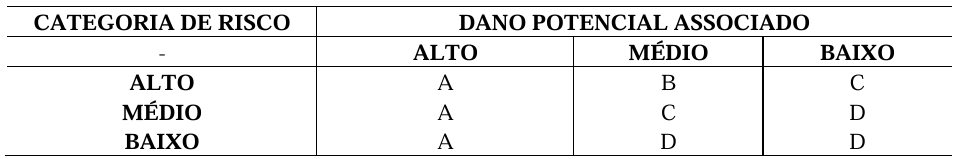
\includegraphics[width=\textwidth]{image27_matriz_de_classificacao_cri_e_dpa_ana.png}
    \caption{Matriz de classificação de barragens quanto ao risco e dano potencial associado}
    \label{fig:matriz_classificacao_ana}
    \fonte{\cite{moecke2019} de acordo com Resolução nº 236 - ANA}
\end{figure}

As Resoluções nº 91/2012 e nº 236/2017 da Agência Nacional de Águas (ANA) estabeleceram diretrizes específicas para a elaboração do Plano de Segurança de Barragens (PSB), diferenciando as exigências conforme a classificação de risco de cada estrutura. Neste contexto regulatório, as barragens enquadradas nas classes de risco ``A'' ou ``B'' devem atender não apenas aos requisitos documentais estabelecidos pela Lei nº 12.334/2010, mas também apresentar obrigatoriamente o Plano de Ações Emergenciais (PAE), instrumento complementar que detalha os procedimentos específicos para situações de emergência \cite{moecke2019}.

\subsection{Classificação das barragens de rejeitos}

A classificação de risco das barragens de rejeitos é um processo que envolve a análise minuciosa de diversos fatores técnicos, estruturais e ambientais. Esta avaliação busca identificar potenciais vulnerabilidades e quantificar os riscos associados à estabilidade dessas estruturas complexas e críticas \cite{cruz2024}.

No Brasil, após os desastres de Mariana e Brumadinho em Minas Gerais, houve significativas mudanças nas leis e normas relacionadas à segurança de barragens, tornando os processos de classificação e monitoramento mais rigorosos \cite{geoscan2020}.

A classificação de risco é aplicada para avaliar sistematicamente os riscos relacionados à estabilidade e segurança das barragens de rejeitos, analisando múltiplos elementos como geometria da barragem, método construtivo empregado, características específicas do rejeito armazenado, condições operacionais e sistemas de drenagem implementados. Estes parâmetros, quando avaliados em conjunto, permitem categorizar as estruturas em diferentes níveis de risco, estabelecendo prioridades para ações de monitoramento e intervenção \cite{cruz2024}.

A Agência Nacional de Mineração (ANM) implementou o Sistema Integrado de Gestão de Barragens de Mineração (SIGBM) como ferramenta para gerenciamento e classificação das barragens de rejeitos no Brasil. Suas principais funcionalidades incluem o Cadastro Nacional de Barragens de Mineração, onde empreendedores registram informações detalhadas sobre suas estruturas, como categoria de risco, dano potencial associado, altura, volume e método construtivo. O sistema também permite o envio de documentos obrigatórios, como a Declaração de Condição de Estabilidade (DCE) e a Declaração de Conformidade e Operacionalidade do Plano de Ação de Emergência para Barragens de Mineração (PAEBM). Além disso, o SIGBM oferece painéis interativos com mapas georreferenciados e análises estatísticas, desenvolvidos com ferramentas de Business Intelligence (BI), proporcionando uma visualização clara e atualizada da situação das barragens. Essas funcionalidades visam aumentar a transparência, padronizar procedimentos fiscalizatórios e promover a segurança das barragens de mineração em todo o território nacional \cite{anmsistema2020}.

Buscando aprimorar a classificação e a gestão de risco, pesquisas contemporâneas exploram metodologias baseadas em dados disponíveis. Cruz \cite{cruz2024} propôs uma metodologia de classificação de barragens de mineração utilizando dados do Sistema Integrado de Gestão de Barragens de Mineração (SIGBM) da ANM. Esta metodologia adaptou conceitos de trabalhos anteriores com o objetivo de criar uma ferramenta para categorizar riscos e auxiliar na priorização da fiscalização pela ANM. A proposta visou quantificar a vulnerabilidade, o potencial de risco e a consequência de um evento indesejado utilizando informações reportadas no SIGBM.

A avaliação de risco em barragens de rejeitos constitui um processo complexo que considera múltiplos fatores para determinar a vulnerabilidade e o potencial de danos dessas estruturas críticas \cite{cruz2024}. Este processo analítico baseia-se na investigação sistemática de quatro elementos principais, cada um contribuindo de forma significativa para a compreensão do comportamento estrutural e dos riscos associados a essas obras de engenharia:

\begin{enumerate}
    \item \textbf{Aspectos Geométricos e Construtivos}: A geometria da barragem, incluindo altura, inclinação dos taludes e largura da crista, influencia diretamente sua estabilidade estrutural. Diferentes métodos construtivos (a montante, a jusante ou linha de centro) apresentam níveis variados de segurança, sendo as barragens a montante consideradas potencialmente mais vulneráveis \cite{cruz2024}.
    \item \textbf{Características do Material Armazenado}: As propriedades físicas e químicas dos rejeitos impactam significativamente o comportamento geotécnico da estrutura. Fatores como granulometria, densidade, teor de umidade e potencial de liquefação são avaliados para determinar possíveis mecanismos de falha \cite{cruz2024}.
    \item \textbf{Sistemas de Drenagem e Monitoramento}: A eficiência dos sistemas de drenagem interna e superficial é crucial para controlar a pressão da água nos poros do material, prevenindo instabilidades. Da mesma forma, a existência e funcionalidade de sistemas de monitoramento adequados permitem a detecção precoce de anomalias \cite{cruz2024}.
    \item \textbf{Condições Operacionais}: As práticas de operação, incluindo velocidade de alteamento, controle do nível freático e manutenção preventiva, influenciam diretamente a segurança da estrutura ao longo do tempo \cite{cruz2024}.
\end{enumerate}

A metodologia desenvolvida por \citeonline{cruz2024} empregou a Análise Hierárquica de Processos (AHP) para atribuir pesos a parâmetros relevantes (Design, Auscultação e Severidade) com base no julgamento de especialistas em segurança de barragens da ANM. A Escala Fundamental de Saaty foi utilizada para converter comparações paritárias em valores numéricos. As notas para os atributos foram extraídas ou adaptadas dos dados do SIGBM, permitindo uma classificação quantitativa do risco.

A aplicação da metodologia de \citeonline{cruz2024} a 203 barragens em Minas Gerais resultou em uma distribuição de níveis de risco, com a maioria classificada como Baixo (79,4\%) ou Moderado (13,8\%), e uma parcela menor como Alto (4,4\%) ou Muito Alto (2,4\%).

A análise dos dados do SIGBM no estudo de \citeonline{cruz2024} identificou que 25\% das barragens analisadas careciam de informações sobre compactação em seus dados de Design, e 38\% estavam fundadas em solo residual/aluvião. Quanto aos dados de Auscultação (inspeções regulares), 50,24\% das barragens apresentaram algum tipo de ocorrência, sendo percolação, drenagem superficial e deterioração dos taludes as mais frequentes.

A adequada classificação de risco das barragens de rejeitos é fundamental para orientar as ações de gestão de segurança, estabelecendo prioridades de intervenção e definindo a frequência e abrangência das inspeções necessárias. Estruturas classificadas como de alto risco demandam monitoramento mais intensivo e medidas preventivas mais rigorosas \cite{geoscan2020, cruz2024}.

Apesar dos avanços nos sistemas de classificação, a gestão de segurança em barragens de rejeitos apresenta limitações substanciais que comprometem a eficácia dos sistemas de classificação existentes. A complexidade dos processos geotécnicos e hidrológicos, aliada à escassez de dados técnicos confiáveis, constitui obstáculo fundamental para avaliações precisas de risco estrutural. A heterogeneidade dos métodos construtivos empregados e as características específicas dos rejeitos minerais em diferentes localidades impossibilitam a implementação de sistemas padronizados de classificação, conforme evidenciado pela diversidade de abordagens regulamentares adotadas internacionalmente \cite{cruz2024}.

Adicionalmente, as mudanças climáticas intensificam eventos meteorológicos extremos, introduzindo variáveis imprevistas nos cálculos de estabilidade estrutural. A incorporação de critérios socioambientais representa desafio adicional, uma vez que as metodologias tradicionais de avaliação focam predominantemente em aspectos técnicos, negligenciando impactos potenciais sobre comunidades locais e ecossistemas circundantes. Essa limitação metodológica evidencia a necessidade de desenvolvimento de frameworks integrados que contemplem múltiplas dimensões de risco, conforme destacado por \citeonline{cruz2024} e \citeonline{moecke2019}.

\subsection{Panorama Atual de Classificação das Barragens de Mineração}

A gestão da segurança de barragens de mineração representa um pilar fundamental para a sustentabilidade da indústria extrativa, exigindo monitoramento contínuo e regulamentação rigorosa. O ``Relatório Mensal - Barragens de Mineração - Fevereiro 2025'' da \citeonline{anm2025boletim} oferece um panorama atualizado da situação dessas estruturas no Brasil, detalhando o número de barragens cadastradas, sua classificação de risco, níveis de emergência declarados e as atividades de fiscalização realizadas. Este documento, elaborado pela Superintendência de Segurança de Barragens de Mineração da ANM, baseia-se em dados atualizados em tempo real e disponíveis no Sistema Integrado de Gestão de Segurança de Barragens de Mineração (SIGBM) Público, refletindo as atualizações ocorridas no intervalo de 02/02/2025 a 05/03/2025. A análise desses dados permite uma compreensão da dinâmica do setor e dos desafios regulatórios e operacionais enfrentados, preparando o terreno para uma investigação mais aprofundada sobre a eficácia das políticas de segurança vigentes \cite{anm2025boletim}.

Segundo a \citeonline{anm2025boletim}, o país contava, em março de 2025, com 917 barragens de mineração cadastradas no Sistema Integrado de Gestão de Segurança de Barragens de Mineração (SIGBM), das quais 467 estavam enquadradas na Política Nacional de Segurança de Barragens (PNSB). Esta configuração representa aproximadamente 51\% do total de estruturas sob supervisão direta da política nacional, evidenciando a magnitude do desafio regulatório enfrentado pelo setor. A distribuição geográfica e os níveis de risco associados a essas estruturas constituem elementos fundamentais para compreender as dinâmicas regionais de segurança mineral \cite{anm2025boletim}.

Lista – Dados Consolidados do Cadastro Nacional:
\begin{itemize}
    \item Total de barragens cadastradas: 917
    \item Barragens inseridas na PNSB: 467 (51\%)
    \item Barragens não inseridas na PNSB: 450 (49\%)
    \item Período de análise: 02/02/2025 a 05/03/2025
\end{itemize}

A análise da distribuição geográfica das barragens de mineração (Figura~\ref{fig:distribuicao_barragens_marco_2025}) revela concentrações específicas que refletem a geografia mineral brasileira e suas tradições extrativas históricas. A análise por estados revela que Minas Gerais concentra o maior número de barragens de mineração em função de sua vocação minerária centenária e da presença do Quadrilátero Ferrífero. O Mato Grosso apresenta-se como segunda região de maior concentração, impulsionado pela expansão da mineração aurífera e pela presença significativa de pequenos empreendimentos, seguido por Pará, Bahia e São Paulo, refletindo a histórica predominância da atividade mineradora nessas regiões \cite{anm2025boletim}.

\begin{figure}[htbp]
    \centering
    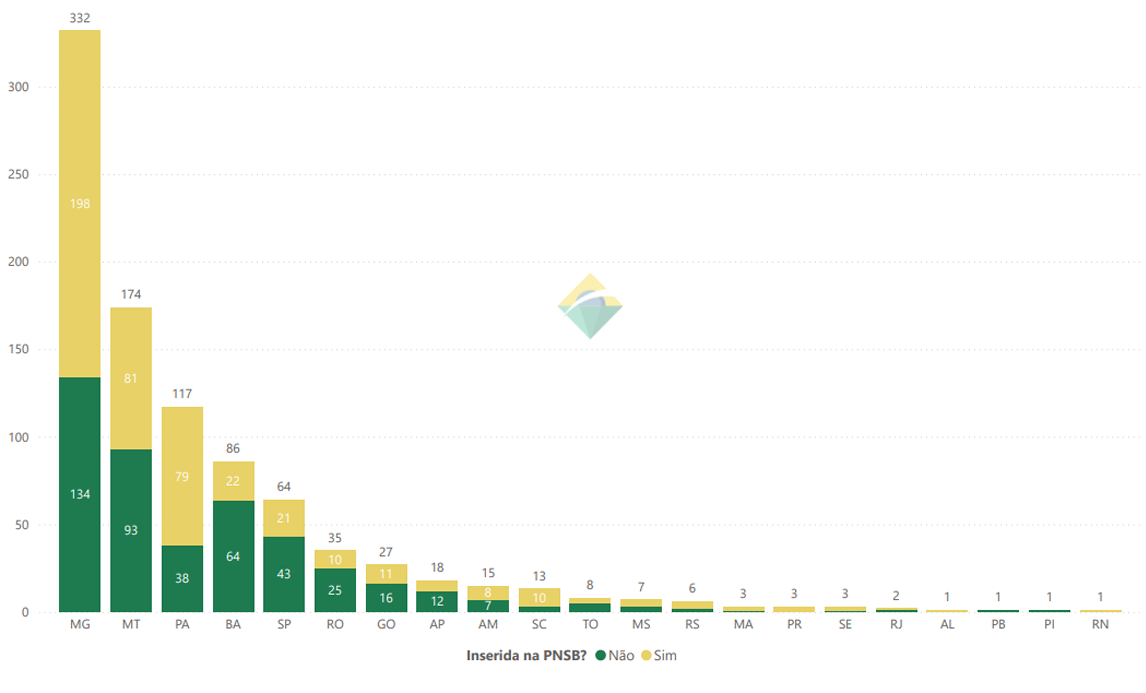
\includegraphics[width=0.8\textwidth]{image28_distribuicao_barragens_marco_2025.png}
    \caption{Distribuição das barragens cadastradas no SIGBM em 05/03/2025.}
    \label{fig:distribuicao_barragens_marco_2025}
    \fonte{\cite{anm2025boletim}}
\end{figure}

\subsection{Categoria de Risco das Barragens}

A Categoria de Risco (CRI) é um indicador crucial na avaliação da segurança de barragens, determinando o nível de atenção regulatória e as exigências de monitoramento para as estruturas enquadradas na PNSB. As barragens inseridas na PNSB estão classificadas em relação à Categoria de Risco - CRI de acordo com a Figura~\ref{fig:distribuicao_barragens_classificacao_cri} e a distribuição nacional das barragens por estado e CRI (Figura~\ref{fig:distribuicao_barragens_classificacao_cri_estado}) mostra a concentração de estruturas em diferentes categorias nas principais regiões mineradoras do Brasil \cite{anm2025boletim}.

\begin{figure}[htbp]
    \centering
    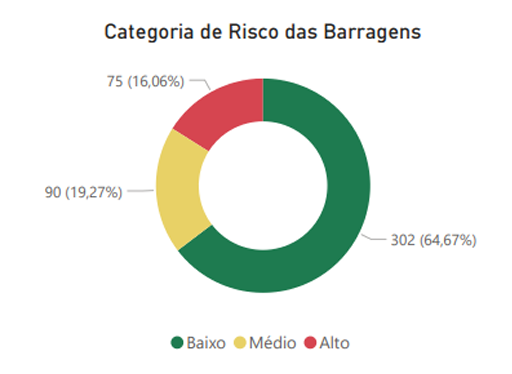
\includegraphics[width=0.8\textwidth]{image29_distribuicao_barragens_classificacao_cri.png}
    \caption{Distribuição de barragens cadastradas de acordo com sua classificação de CRI.}
    \label{fig:distribuicao_barragens_classificacao_cri}
    \fonte{\cite{anm2025boletim}}
\end{figure}

\begin{figure}[htbp]
    \centering
    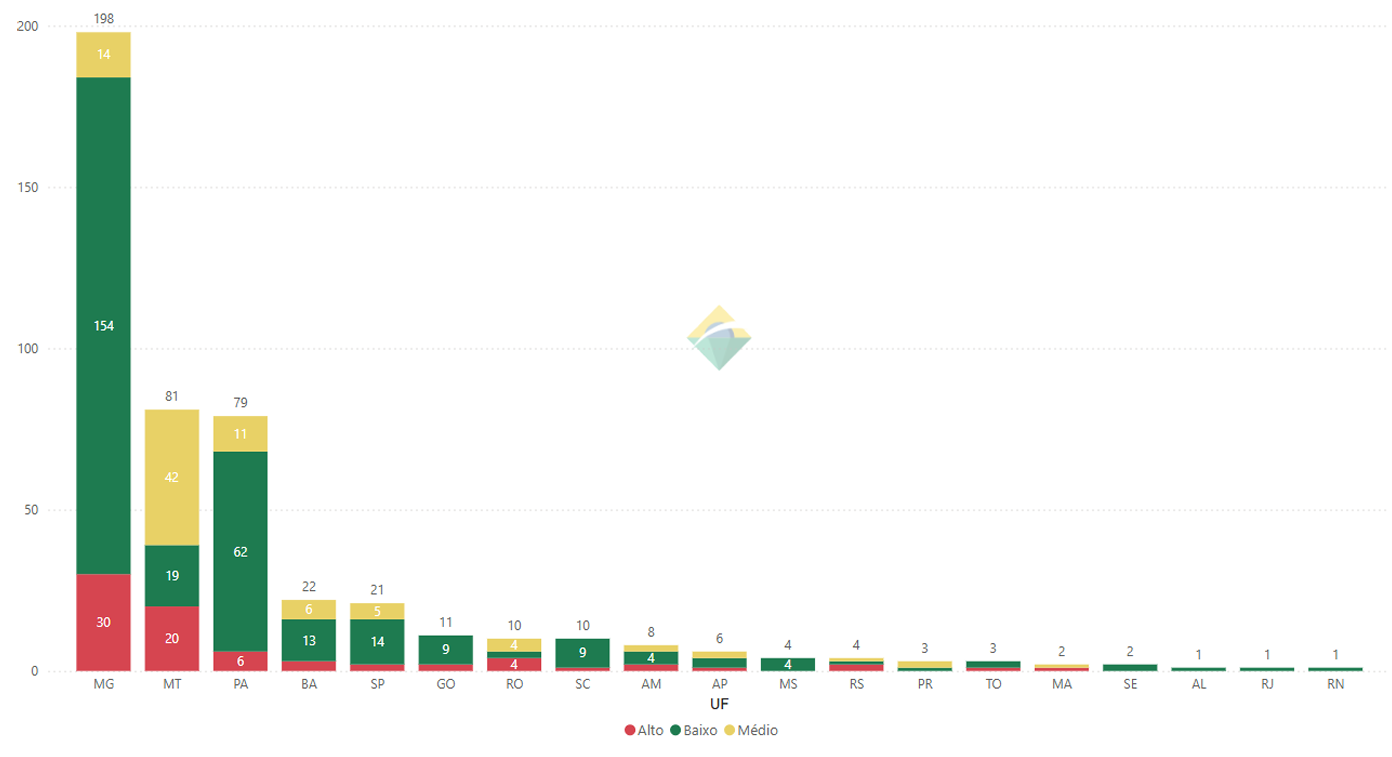
\includegraphics[width=0.8\textwidth]{image30_distribuicao_barragens_classificacao_cri_estado.png}
    \caption{Distribuição das barragens inseridas na PNSB por estado, segundo a classificação de CRI.}
    \label{fig:distribuicao_barragens_classificacao_cri_estado}
    \fonte{\cite{anm2025boletim}}
\end{figure}

Conforme ilustrado nas Figuras~\ref{fig:distribuicao_barragens_classificacao_cri} e~\ref{fig:distribuicao_barragens_classificacao_cri_estado}, Minas Gerais se destaca não apenas em quantidade, mas também em número absoluto de barragens classificadas como CRI alto, o que se explica pela presença de grandes complexos mineradores e pelo histórico de acidentes recentes, como os de Mariana e Brumadinho. O Pará, por sua vez, apresenta um perfil de barragens com maior proporção de risco médio e baixo, em função do predomínio de estruturas mais recentes e de métodos construtivos alternativos, como o empilhamento a seco. Mato Grosso e Goiás, embora possuam menor número absoluto, têm apresentado crescimento nas reclassificações para risco alto, especialmente em barragens de pequeno e médio porte operadas por empresas de menor capitalização \cite{anm2025boletim}.

O mês de fevereiro de 2025 testemunhou alterações significativas na classificação de risco de 14 barragens, revelando a natureza dinâmica dos sistemas de avaliação e as consequências das mudanças regulamentares recentes. Entretanto, o relatório destaca um fator regulatório preponderante no aumento do número de barragens classificadas com CRI Alto: a implementação de uma regra no SIGBM conforme o inciso II do § 1º do Art. 5º da Resolução ANM nº 95/2022, alterada pela Resolução ANM nº 175/2024. Esta norma estabelece que a falta de envio da Declaração de Condição de Estabilidade (DCE) da Revisão Periódica de Segurança de Barragem resulta na classificação automática da barragem como CRI Alto e, consequentemente, em nível de emergência 1. Por exemplo, a barragem "Bacia de Acumulação 01", em Urussanga/SC, passou de risco baixo para alto, enquanto a "Barragem B", em Patos de Minas/MG, foi reclassificada de alto para baixo risco. Essas alterações demonstram a dinamicidade do sistema de classificação, que responde tanto a fatores técnicos quanto administrativos \cite{anm2025boletim}.

Essa nova regra foi incorporada ao SIGBM em 13/02/2025, após o término do prazo de seis meses para os empreendedores se adequarem, impactando diretamente as classificações e elevando o número de barragens em CRI Alto. A alteração da Categoria de Risco de Baixo ou Médio para Alto para diversas barragens demonstra o efeito imediato dessa medida regulatória, sublinhando a importância do cumprimento dos prazos de entrega documental para a manutenção de uma classificação de risco adequada. A evolução do número de barragens em cada categoria de risco ao longo dos últimos 12 meses (Figura \ref{fig:evolucao_classificacao}) ilustra essa dinâmica e as tendências temporais na classificação de segurança das estruturas \cite{anm2025boletim}.

\begin{figure}[htbp]
    \centering
    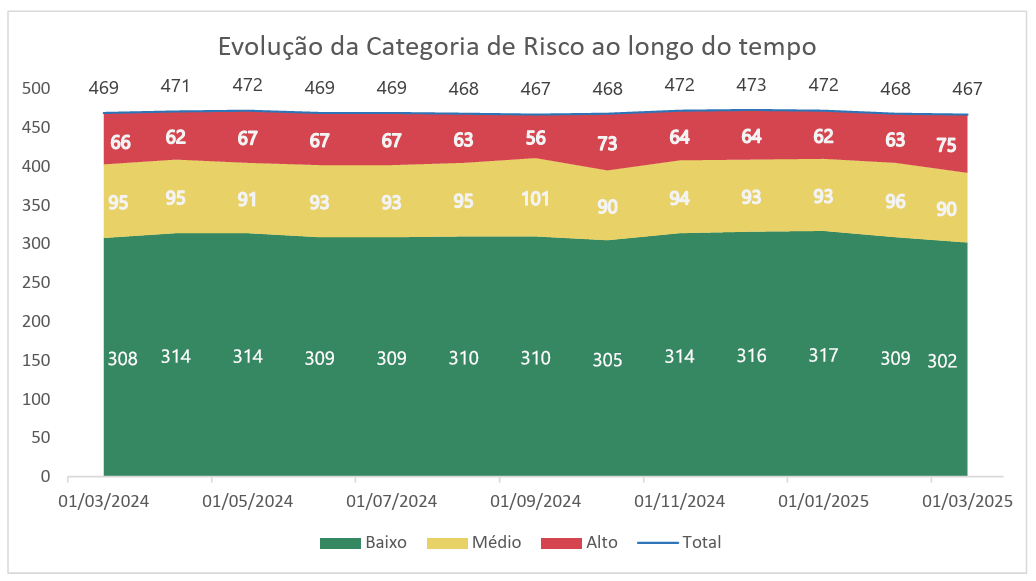
\includegraphics[width=0.8\textwidth]{image31_evolucao_classificacao_12_meses.png}
    \caption{Evolução da classificação de CRI ao longo dos últimos 12 meses.}
    \label{fig:evolucao_classificacao}
    \fonte{ANM (2025)}
\end{figure}

Complementar à classificação de risco, a situação de alerta ou emergência declarada indica um estado de atenção ou criticidade que demanda ações imediatas por parte dos empreendedores e acompanhamento intensivo pela ANM. Em março de 2025, 104 barragens se encontravam nessa situação, distribuídas em diferentes níveis de emergência (Nível 1, Nível 2 e Nível 3) ou em situação de alerta. A distribuição dessas barragens por estado (Figura \ref{fig:distribuicao_alerta}) revela que a maioria se localiza em Minas Gerais, Mato Grosso, Pará e Rondônia \cite{anm2025boletim}.

\begin{figure}[htbp]
    \centering
    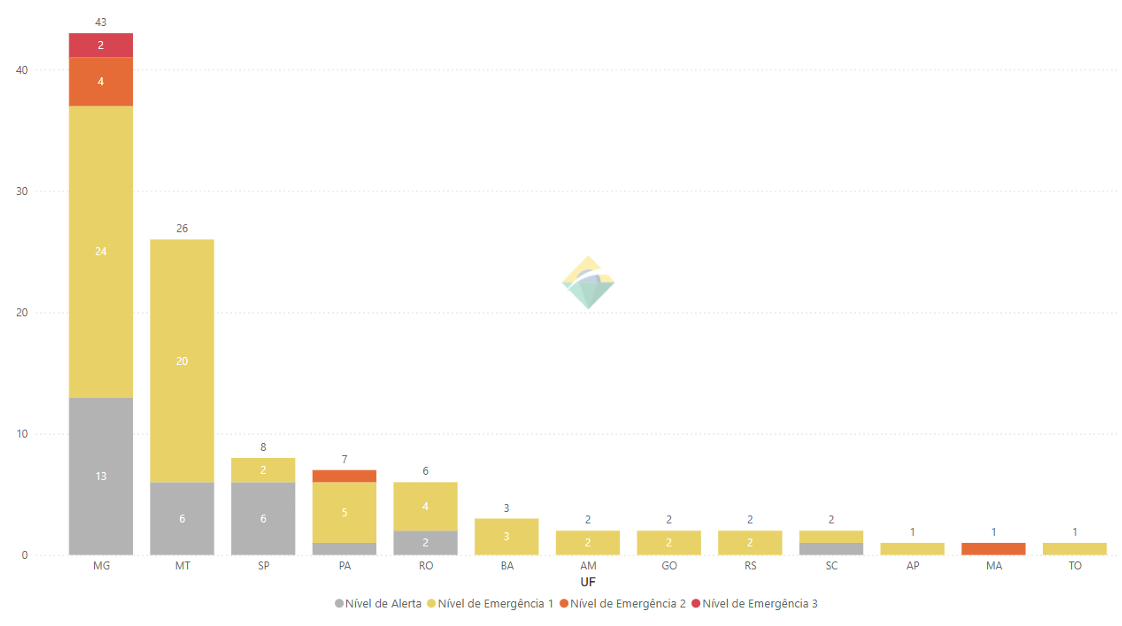
\includegraphics[width=0.8\textwidth]{image32_distribuicao_barragens_nivel_alerta.png}
    \caption{Distribuição das barragens em nível de alerta ou emergência por estado em 05/03/2025.}
    \label{fig:distribuicao_alerta}
    \fonte{ANM (2025)}
\end{figure}

A evolução do número de barragens em nível de alerta ou emergência ao longo dos últimos meses revela um aumento significativo a partir da implementação das novas regras de classificação automática por descumprimento de obrigações legais. Esse fenômeno, embora possa inflar artificialmente o número de barragens em emergência, reflete a importância da gestão documental e da cultura de segurança nas empresas mineradoras. Destaca-se que apenas duas barragens, ambas em Minas Gerais, encontravam-se em Nível de Emergência 3, o mais crítico, enquanto seis estavam em Nível 2, distribuídas entre Minas Gerais, Pará e Maranhão. O Nível de Emergência 1 é o nível inicial dentro do estado de emergência declarada, frequentemente acionado por não conformidades regulatórias ou pela necessidade de investigações mais aprofundadas, mesmo na ausência de um risco estrutural imediato; 67 barragens se encontram em Nível 1 \cite{anm2025boletim}.

Lista – Barragens em Nível de Emergência 3 (março/2025):
\begin{itemize}
    \item Barragem Serra Azul (ArcelorMittal Brasil S.A.) – Itatiaiuçu/MG
    \item Forquilha III (Vale S.A.) – Ouro Preto/MG
\end{itemize}

Lista – Barragens em Nível de Emergência 2 (março/2025):
\begin{itemize}
    \item Bacia do Castanheira (Buritirama Mineração S.A.) – Marabá/PA
    \item Barragem do Vené (Mineração Aurizona S/A) – Godofredo Viana/MA
    \item Forquilha I, Forquilha II, Sul Superior, Xingu (Vale S.A.) – Ouro Preto, Barão de Cocais, Mariana/MG
\end{itemize}

A presença de empreendedores como VALE S.A. e BURITIRAMA MINERACAO S.A. na lista dos níveis de emergência mais altos aponta para a necessidade de atenção contínua, independentemente do porte da empresa, e destaca a responsabilidade dos grandes players do setor na gestão da segurança \cite{anm2025boletim}.

A recorrência de situações de emergência em barragens localizadas em Minas Gerais, como exemplificado acima, está associada tanto ao envelhecimento das estruturas quanto à complexidade geotécnica da região, marcada por solos residuais e regimes pluviométricos variáveis. Por outro lado, em estados como Pará e Mato Grosso, o desafio reside na rápida expansão da atividade mineradora e na necessidade de adaptação das pequenas empresas às exigências regulatórias mais rigorosas. A seguir, será discutida a evolução temporal do número de barragens em situação de emergência, com ênfase nas tendências observadas nos últimos anos \cite{anm2025boletim}.

A evolução do número de barragens em nível de alerta ou emergência ao longo dos últimos 24 meses, conforme ilustrado na Figura 6 do relatório da ANM (2025), revela um aumento significativo a partir da implementação das novas regras de classificação automática por descumprimento de obrigações legais. Esse fenômeno, embora possa inflar artificialmente o número de barragens em emergência, reflete a importância da gestão documental e da cultura de segurança nas empresas mineradoras. Em contrapartida, observa-se uma tendência de redução dos casos mais críticos (Nível 2 e 3), resultado do esforço conjunto entre órgãos fiscalizadores e setor produtivo para descomissionamento de estruturas instáveis e adoção de tecnologias mais seguras, como o empilhamento a seco. A análise desses dados evidencia que a gestão de barragens de mineração no Brasil é um processo dinâmico, que exige constante atualização normativa e investimento em capacitação técnica. No próximo parágrafo, serão sugeridas imagens e gráficos que podem enriquecer a compreensão do tema \cite{anm2025boletim}.

\subsection{Risco: Severidade x Probabilidade}
\label{subsec:risco}

O conceito de risco é fundamental na gestão de segurança, sendo definido como a combinação entre a probabilidade de ocorrência de um evento perigoso e a severidade das consequências desse evento. A probabilidade refere-se à chance estimada de que o risco se concretize, enquanto a severidade diz respeito ao grau de dano ou prejuízo que o evento pode causar, variando de lesões leves até consequências fatais. Essa relação é frequentemente expressa matematicamente como o produto entre probabilidade e severidade, formando o chamado nível de risco, ferramenta essencial para priorização e tomada de decisões em ambientes ocupacionais e de saúde \cite{sistemaeso2021avaliacao, sistemaeso2021matriz, segurancatemfuturo}.

A quantificação de riscos no setor minerário baseia-se fundamentalmente na relação matemática entre probabilidade e severidade das consequências. O setor de mineração quantifica o risco através do produto da probabilidade pela severidade, sendo a probabilidade definida pela soma de quatro componentes principais que caracterizam diferentes cenários de falha \cite{iramina2009}. Esta abordagem sistemática permite uma avaliação mais precisa dos perigos inerentes às operações de extração mineral, considerando variáveis como condições geotécnicas, processos operacionais e fatores ambientais. A metodologia de análise RBPS exemplifica essa abordagem, permitindo aferir a probabilidade de um rompimento e suas prováveis consequências a partir da formulação de quatro cenários mais frequentes: estático, hidrológico, sísmico e operação e manutenção \cite{conceicao2018}.

A definição operacional de risco na mineração transcende a simples multiplicação de fatores, incorporando aspectos multidimensionais que afetam a segurança operacional. Segundo \citeonline{iramina2009}, os riscos presentes nas operações unitárias do processo produtivo de pedra britada em uma mina a céu aberto devem ser sistematicamente identificados e controlados através de programas estruturados de gerenciamento. Esta perspectiva multifacetada reconhece que os riscos minerários envolvem não apenas aspectos técnicos, mas também dimensões sociais, ambientais e econômicas que influenciam tanto a probabilidade quanto a severidade dos eventos adversos.

As metodologias para determinação da probabilidade de ocorrência em operações minerárias empregam abordagens tanto qualitativas quanto quantitativas. A APR e a BTA constituem ferramentas fundamentais para identificação dos cenários potenciais indesejáveis, causas e efeitos potenciais, gradação dos efeitos e estimativa de probabilidade \cite{vilaca2021}. Essas metodologias permitem classificar eventos conforme sua probabilidade temporal, estabelecendo categorias que variam desde eventos improváveis até aqueles com possibilidade de ocorrência em períodos específicos de 5 a 10 anos \cite{vilaca2021}.

A quantificação probabilística na mineração deve considerar a variabilidade temporal e espacial dos fatores de risco presentes nas diferentes operações. Os principais riscos envolvidos na mineração incluem soterramento, detonação, contato com substâncias químicas, explosões de gases, desabamentos de minas, trabalho em espaço confinado e exposição ao ruído \cite{vendrame2023}. Cada uma dessas categorias de risco apresenta características probabilísticas distintas, influenciadas por fatores como condições geológicas, métodos de extração empregados, condições climáticas e qualidade dos procedimentos operacionais. A metodologia RBPS demonstra essa complexidade ao considerar múltiplos cenários de falha, em que diferentes barragens podem apresentar índices de falha com variação significativa, como observado em estudos que identificaram valores entre 375,66 e 455,18 pontos para diferentes estruturas \cite{conceicao2018}.

A severidade das consequências em eventos minerários manifesta-se através de múltiplas dimensões que afetam trabalhadores, comunidades e meio ambiente. A avaliação da severidade considera consequência máxima ou alta para segurança, meio ambiente, social, legal, financeiro e reputacional \cite{vilaca2021}, estabelecendo uma classificação multidimensional que transcende os impactos puramente operacionais. Esta abordagem sistêmica reconhece que eventos adversos na mineração podem gerar consequências em cascata, afetando desde a integridade física dos trabalhadores até aspectos socioambientais mais amplos. O estudo de barragens minerárias exemplifica essa complexidade, demonstrando que uma única estrutura pode potencialmente afetar 12.900 pessoas, resultando em um Índice de Risco Total de 969,20 pontos \cite{conceicao2018}.

A graduação da severidade requer metodologias específicas que considerem tanto os efeitos imediatos quanto os impactos de longo prazo. As operações de desmonte de rochas ilustram essa complexidade, envolvendo riscos como explosões acidentais, vibrações sísmicas, lançamento de fragmentos e exposição a produtos químicos perigosos \cite{vendrame2023}. Cada uma dessas consequências apresenta características distintas em termos de área de impacto, duração dos efeitos e possibilidade de reversão dos danos causados. A classificação de uma barragem como possível causadora de danos extremos \cite{conceicao2018} exemplifica como a severidade pode atingir níveis catastróficos, justificando a implementação de medidas de controle proporcionalmente rigorosas.

Os estudos contemporâneos demonstram a aplicação prática das metodologias de avaliação de risco em diferentes contextos minerários brasileiros. A pesquisa realizada em pedreiras da região metropolitana de São Paulo evidencia como a identificação dos principais riscos associados às operações de perfuração, desmonte, carregamento e transporte, britagem e peneiramento \cite{iramina2009} pode ser sistematicamente conduzida através de medições de campo e análise de registros empresariais. Esta abordagem empírica permite não apenas a identificação dos riscos, mas também a validação das estimativas probabilísticas através de dados operacionais reais. A aplicação da metodologia em seis barragens do estado do Pará demonstra a viabilidade de comparações sistemáticas entre diferentes estruturas, permitindo a priorização de ações de controle baseada em critérios objetivos \cite{conceicao2018}.

As metodologias modernas de avaliação de risco, fundamentadas em normas como a ISO 31000, estabelecem um método para identificar antecipadamente os riscos inerentes a cada organização, avaliar a probabilidade e severidade de incidentes e implementar medidas de controle eficientes \cite{cruz2024iso}. Esta norma busca servir como guia de gestão de riscos, fornecendo uma abordagem clara e comum que pode ser aplicada em diversos ramos, auxiliando os tomadores de decisão a terem escolhas corretas e conscientes, priorizar ações e identificar soluções adequadas \cite{ministeriotransportes2018}.

A implementação de sistemas de gestão de risco baseados na ISO 31000 exemplifica a evolução das práticas contemporâneas na mineração. O estudo de taludes em minerodutos demonstra como a aplicação sistemática de conceitos da ISO 31000, com estabelecimento do contexto, processos de avaliação de riscos e tratamento dos riscos, pode resultar em reduções significativas do grau de risco, passando de 22 (Alto) para 19 (Significativo) \cite{vilaca2021}. Esta redução quantitativa ilustra a eficácia das metodologias estruturadas de gestão de risco quando adequadamente implementadas. A transformação da probabilidade de "possível" para "improvável" demonstra como intervenções técnicas específicas podem alterar fundamentalmente o perfil de risco operacional \cite{vilaca2021}.

\section{Legislação ambiental: população e ambiente (Brasil x Exterior)}
\label{sec:legislacao}

A primeira fase da regulamentação minerária brasileira caracterizou-se pela vinculação entre propriedade do solo e subsolo estabelecida pela Constituição republicana de 1891. Essa Constituição determinou que a propriedade do subsolo estava vinculada à propriedade do solo, refletindo uma concepção liberal de direitos proprietários típica do período \cite{mme2025linha}.

Tal abordagem permitia aos proprietários rurais a exploração irrestrita dos recursos minerais encontrados em suas terras, sem considerações específicas sobre impactos ambientais ou interesse nacional. Posteriormente, o marco de 1907 representou uma mudança institucional significativa com a criação e instalação do Serviço Geológico e Mineralógico do Brasil, evidenciando a necessidade crescente de conhecimento técnico-científico sobre os recursos minerais nacionais \cite{mme2025linha}.

O período getulista marcou uma ruptura fundamental na concepção jurídica dos recursos minerais, estabelecendo o controle estatal sobre o subsolo nacional. Em 1930, foi criada a Companhia Petróleos do Brasil, sinalizando a intenção governamental de assumir maior protagonismo no setor energético \cite{mme2025linha}. 

O presidente Getúlio Vargas defendeu enfaticamente \textit{``a necessidade de se nacionalizarem as reservas minerais do Brasil''} em 1931, promulgando decretos que \textit{``suspenderam a alienação ou oneração de qualquer jazida mineral''} \cite{mme2025linha}. A Constituição de 1934 consolidou juridicamente esta transformação ao separar definitivamente \textit{``as propriedades do solo e do subsolo''}, estabelecendo o controle estatal sobre os recursos minerais \cite{mme2025linha}.

Esta mudança paradigmática culminou com a criação do DNPM pelo Decreto n. 23.979, de 8 de março de 1934, institucionalizando a gestão estatal dos recursos minerais e preparando o caminho para regulamentações mais específicas sobre atividades extrativas \cite{mme2025linha}.

A Constituição outorgada durante o Estado Novo aprofundou o controle nacionalista sobre a mineração, restringindo significativamente a participação estrangeira no setor. A Constituição de 1937 estabeleceu que \textit{``o aproveitamento de jazidas minerais passou a ser autorizado somente a brasileiros ou empresas constituídas por brasileiros''}, consolidando a política nacionalista iniciada na década anterior \cite{mme2025linha}.

Em 1938, foi criado o Conselho Nacional do Petróleo (CNP), que inicialmente mantinha \textit{``livre a iniciativa de pesquisa e exploração de petróleo e gás natural''}, mas posteriormente promoveu \textit{``a nacionalização do refino de petróleo e a regulação da importação e do transporte''} \cite{mme2025linha}.

A Lei Constitucional nº 4, de 19 de junho de 1940, introduziu \textit{``a cobrança de um imposto único sobre minerais no Brasil, de competência da União''}, instituindo tributação específica \textit{``sobre o carvão nacional, os combustíveis e os lubrificantes de qualquer origem''} \cite{mme2025linha}. Paralelamente, o Decreto-lei nº 1.985, de 29 de março de 1940, denominado Código de Minas, definiu formalmente \textit{``os direitos sobre as jazidas''} minerais, estabelecendo as bases jurídicas que posteriormente influenciariam a legislação ambiental \cite{mme2025linha}.

A partir da década de 1970, observou-se uma intensificação da preocupação governamental e jurídica relacionada à preservação ambiental e à qualidade de vida, motivada pela percepção dos danos ambientais crescentes e pela compreensão de que os recursos naturais são limitados.

No âmbito internacional, a Conferência das Nações Unidas sobre Meio Ambiente Humano, ocorrida em Estocolmo em junho de 1972, simbolizou a formalização dessa nova perspectiva, sendo sua declaração reconhecida como o marco fundador do Direito Ambiental em escala global. O documento estabeleceu o direito a um ambiente ecologicamente equilibrado como direito essencial, colocando-o no mesmo patamar de outros direitos fundamentais como liberdade e igualdade, conforme expresso no Princípio nº 1, que reconhece o direito humano fundamental a condições de vida adequadas em ambiente de qualidade, além da responsabilidade de preservá-lo para as futuras gerações. Simultaneamente à Conferência de Estocolmo, foi instituído o PNUMA (Programa das Nações Unidas para o Meio Ambiente), órgão do sistema ONU destinado ao acompanhamento das iniciativas ambientais nacionais e internacionais no contexto do desenvolvimento sustentável \cite{barros2017legislacao}.

No Brasil, a Lei Federal nº 6.938/1981 \cite{brasil1981lei6938}, que instituiu a PNMA, estabeleceu instrumentos fundamentais para o controle ambiental das atividades minerárias. A Política Nacional do Meio Ambiente \textit{``tem por objetivo a preservação, melhoria e recuperação da qualidade ambiental, além de prever sanções em caso de não cumprimento de medidas necessárias à preservação ambiental''} \cite{jazida2022leis}.

Esta legislação introduziu a necessidade de autorizações emitidas pelo governo para a realização de estudos ambientais e obtenção de licenças vinculadas ao processo de mineração \cite{jazida2022leis}. A PNMA regulamentou especificamente os processos de mineração, enfatizando no parágrafo 2º que aquele que explorar recursos minerais fica obrigado a recuperar o meio ambiente degradado, de acordo com solução técnica exigida pelo órgão público competente, na forma da lei. As sanções previstas pela PNMA incluem desde a perda de incentivos fiscais à suspensão das atividades, demonstrando a seriedade do compromisso legal com a proteção ambiental \cite{jazida2022leis}.

A década de 1980 marcou a consolidação dos instrumentos de avaliação de impacto ambiental como ferramentas centrais da governança ambiental minerária. A Resolução CONAMA nº 001/1986 estabeleceu no Brasil a obrigatoriedade do EIA e do RIMA para atividades de extração mineral, definindo metodologias específicas para identificação, quantificação e mitigação dos impactos ambientais \cite{conama1986resolucao001}.

Paralelamente, a legislação internacional evoluiu com a adoção de protocolos de avaliação ambiental mais rigorosos, exemplificados pela Diretiva 85/337/CEE da União Europeia, que estabeleceu padrões harmonizados para avaliação de impactos de projetos de desenvolvimento, incluindo operações de mineração \cite{eu1985diretiva337}.

O final da década de 1980 e início dos anos 1990 foram caracterizados pela introdução de mecanismos de responsabilização civil e criminal por danos ambientais na mineração. A Constituição Federal de 1988 \cite{brasil1988constituicao} representou um divisor de águas ao estabelecer princípios fundamentais para a conciliação entre atividade minerária e proteção ambiental.

O artigo 176 da Constituição Federal reafirmou que o subsolo é propriedade da União, mantendo o controle estatal sobre os recursos minerais estabelecido nas décadas anteriores \cite{brasil1988constituicao}. Já o artigo 225 introduziu o direito fundamental ao \textit{``meio ambiente ecologicamente equilibrado, bem de uso comum do povo e essencial à sadia qualidade de vida''}, impondo \textit{``ao Poder Público e à coletividade o dever de defendê-lo e preservá-lo para as presentes e futuras gerações''} \cite{jazida2022leis}.

Este artigo criou também a responsabilidade objetiva para reparação de danos ambientais e tipificou crimes contra o meio ambiente. O parágrafo 2º do artigo 225 estabeleceu especificamente que \textit{``aquele que explorar recursos minerais fica obrigado a recuperar o meio ambiente degradado, de acordo com solução técnica exigida pelo órgão público competente, na forma da lei''} \cite{jazida2022leis}.

A Lei nº 9.605/1998 \cite{brasil1998lei9605}, conhecida como Lei de Crimes Ambientais, especificou as condutas criminosas relacionadas à poluição e degradação ambiental, estabelecendo penalidades que incluem desde multas até prisão para responsáveis por danos em operações minerárias.

Esta legislação \textit{``contempla a esfera penal e dispõe sobre as sanções penais e administrativas decorrentes de condutas e atividades que gerem impacto ou que venham causar qualquer dano ao meio ambiente''} \cite{jazida2022leis}. O artigo 55 da Lei dos Crimes Ambientais estabelece que constitui crime \textit{``executar pesquisa, lavra ou extração de recursos minerais sem a competente autorização, permissão, concessão ou licença, ou em desacordo com a obtida''}, sendo aplicável \textit{``pena de detenção, de seis meses a um ano, e multa''} \cite{brasil1998lei9605}.

A legislação também criminaliza a conduta de quem \textit{``deixa de recuperar a área pesquisada ou explorada, nos prazos fixados pelos órgãos competentes''} \cite{brasil1998lei9605}.

A década de 1990 testemunhou a emergência e consolidação dos sistemas de gestão ambiental como instrumentos centrais da governança minerária sustentável. A publicação da norma ISO 14001 em 1996 estabeleceu padrões internacionais para sistemas de gestão ambiental \cite{abnt2015iso14001}, fornecendo às empresas mineradoras um framework estruturado para identificação, controle e melhoria contínua de seus aspectos e impactos ambientais. 

No contexto regulatório brasileiro, a Resolução CONAMA nº 237/1997 aprimorou os procedimentos de licenciamento ambiental, estabelecendo três modalidades de licenças (prévia, de instalação e de operação) e definindo competências entre os órgãos ambientais federal, estaduais e municipais \cite{conama1997resolucao237}.

O início do século XXI foi marcado pelo fortalecimento dos mecanismos de participação social e transparência nos processos de licenciamento e operação de empreendimentos minerários. A Resolução CONAMA nº 09/1987 \cite{conama1987resolucao9}, posteriormente complementada pela Resolução nº 286/2001 \cite{conama2001resolucao286}, estabeleceu procedimentos específicos para a realização de audiências públicas durante o processo de licenciamento ambiental, garantindo o direito das comunidades afetadas de se manifestarem sobre os projetos propostos.

A primeira década dos anos 2000 testemunhou o desenvolvimento de regulamentações específicas para segurança de barragens de rejeitos minerários, impulsionado por acidentes significativos em diversos países. No Brasil, a Lei nº 12.334/2010 estabeleceu a Política Nacional de Segurança de Barragens (PNSB), definindo critérios de classificação baseados em risco e dano potencial. 

A norma brasileira NBR 13028:2017 complementou esse framework ao estabelecer diretrizes técnicas específicas para elaboração e apresentação de projetos de barragens de rejeitos de mineração, incluindo requisitos para análise de estabilidade, monitoramento e planos de emergência. Internacionalmente, diretrizes como as da International Commission on Large Dams (ICOLD) e padrões da Canadian Dam Association forneceram parâmetros técnicos que influenciaram regulamentações nacionais em diversos países \cite{icold2001tailings, cda2007guidelines}.

A década de 2010 foi caracterizada pela emergência e consolidação dos critérios ESG (Environmental, Social and Governance) como paradigma central da governança empresarial na mineração. Iniciativas como os Princípios do Equador (2003, revisados em 2013 e 2020) estabeleceram critérios socioambientais para financiamento de projetos de grande porte, incluindo operações minerárias, criando incentivos de mercado para adoção de práticas sustentáveis \cite{equator2020principles}.

A regulamentação brasileira incorporou elementos de governança ESG através de normativas da Comissão de Valores Mobiliários (CVM), como a Instrução nº 480/2009, que estabeleceu requisitos de transparência para companhias abertas, incluindo divulgação de riscos socioambientais e práticas de governança corporativa \cite{cvm2009instrucao480}.

Frameworks internacionais como o Global Reporting Initiative (GRI) e o Sustainability Accounting Standards Board (SASB) desenvolveram métricas específicas para o setor minerário, permitindo comparabilidade e benchmarking de desempenho sustentável entre empresas \cite{gri2013mining, sasb2018sustainability}. Conforme destaca a Xenith Consulting \cite{xenith2025esg}, a integração de critérios ESG transformou fundamentalmente a avaliação de projetos minerários, incorporando considerações de longo prazo sobre sustentabilidade e licença social para operar.

\subsection{Estrutura Regulatória Contemporânea}

A estrutura regulatória contemporânea da mineração brasileira centraliza-se na Agência Nacional de Mineração (ANM), criada pela Lei nº 13.575/2017 e instalada em 28 de novembro de 2018 \cite{brasil2017senado}, que consolidou as funções de controle e fiscalização do setor. A atividade de mineração no Brasil é regulamentada pela ANM, sendo uma de suas atribuições dar andamento aos trâmites dos processos minerários \cite{jazida2022leis}.

A ANM administra o conceito de "processo minerário" como uma parcela de terra para a qual o titular reivindicou o direito de desenvolver e extrair um depósito mineral, esclarecendo que este direito não inclui direitos à superfície \cite{jazida2022leis}. A confirmação constitucional de que as jazidas minerais pertencem à União significa que a lavra e pesquisa mineral só poderá ser realizada com a devida autorização da ANM \cite{jazida2022leis}.

A atividade minerária contemporânea engloba vários processos, como pesquisa mineral, estudo de viabilidade econômica, licenciamento ambiental, lavra, beneficiamento, tratamento de rejeitos até o fechamento da mina \cite{jazida2022leis}.

A resposta regulatória aos desastres minerais brasileiros resultou em uma das mais abrangentes reformas normativas da história do setor, promovendo a evolução da regulamentação ambiental minerária brasileira e internacional. A Agência Nacional de Mineração (ANM) promulgou uma série de resoluções técnicas que revolucionaram os padrões de segurança, destacando-se a Resolução ANM nº 4/2019 \cite{anm2019resolucao4}, que proibiu a construção de novas barragens pelo método de alteamento a montante. A Resolução ANM nº 13/2019 \cite{anm2019resolucao13} estabeleceu novos critérios para a Declaração de Condição de Estabilidade (DCE), exigindo análises mais rigorosas de estabilidade estática e dinâmica.

A Lei nº 12.334/2010 criou o Sistema Nacional de Informações sobre Segurança de Barragens (SNISB), centralizando dados sobre todas as estruturas do país e estabelecendo protocolos rigorosos de monitoramento e fiscalização. Internacionalmente, esses eventos estimularam a criação do Global Industry Standard on Tailings Management, desenvolvido conjuntamente pelo International Council on Mining and Metals (ICMM), Programa das Nações Unidas para o Meio Ambiente (PNUMA) e Principles for Responsible Investment (PRI) \cite{icmm2020global}.

Segundo \citeonline{icmm2020global}, os desastres brasileiros expuseram as limitações dos sistemas regulatórios tradicionais e demandaram uma reformulação abrangente dos marcos de governança ambiental na mineração.

\subsection{Tecnologias Emergentes e Inteligência Artificial}

A última década tem sido caracterizada pela crescente integração de tecnologias digitais nos sistemas de governança ambiental minerária. A Resolução ANM nº 95/2022 introduziu o conceito de revisão periódica de segurança obrigatória, com a implementação de sistemas de monitoramento em tempo real de barragens de rejeitos, incluindo instrumentação geotécnica automatizada, sistemas de alerta precoce e plataformas de visualização de dados \cite{anm2022resolucao95}.

Essas normas incorporaram recomendações internacionais das melhores práticas, incluindo diretrizes da International Commission on Large Dams \cite{icold2022tailings} e padrões canadenses de gestão de rejeitos \cite{mac2021guide}.

Tecnologias como sensoriamento remoto por satélite, drones para inspeção ambiental e inteligência artificial para análise preditiva de riscos têm sido progressivamente incorporadas aos marcos regulatórios \cite{darzi2024transformacao}. A União Europeia, por meio do European Green Deal e da taxonomia sustentável, estabeleceu critérios técnicos específicos para classificação de atividades minerárias como ambientalmente sustentáveis, incluindo requisitos para uso de tecnologias de monitoramento avançadas \cite{eu2020taxonomy}.

\section{Acidentes em Mariana e Brumadinho}
\label{sec:acidentes}

Barragens de rejeitos são reservatórios feitos com o objetivo de reter
água e resíduos sólidos resultantes da extração de minérios para que
evite danos ambientais. (OBTER O TEXTO FINAL - RENATA)

\section{Sistema de alerta existentes}
\label{sec:sistema_alerta}

AQUIIIIII

\subsection{Higrômetro de Resistência e seu uso na prevenção de acidentes de barragens}
\label{subsec:higrometro}